\documentclass[citestyle=gb7714-2015, bibstyle=gb7714-2015,lang=cn,14pt,scheme=chinese]{elegantbook}

\title{深度学习模型的学习动态}
\subtitle{xxxxx}

\author{姜广琛}
\institute{西北工业大学}
\date{2025/04/17}
\version{0.1}
% \bioinfo{自定义}{信息}

% \extrainfo{注意:本模板自 2023 年 1 月 1 日开始,不再更新和维护!}

\setcounter{tocdepth}{3}

\logo{logo-blue.png}
\cover{cover.jpg}

% 本文档命令
\usepackage{minted}
\usepackage[linesnumbered,ruled,vlined]{algorithm2e}
\usepackage{subcaption}


% 修改标题页的橙色带
\definecolor{customcolor}{RGB}{32,178,170}
\colorlet{coverlinecolor}{customcolor}
\usepackage{cprotect}

\addbibresource[location=local]{reference.bib} % 参考文献,不要删除
\ExecuteBibliographyOptions{sorting=ynt}

\begin{document}

% \maketitle
\frontmatter

\tableofcontents

\mainmatter%

\chapter{环境设置}

\section{扫地机器人(Sweeping Robot)}

对于扫地机器人的环境,我参考的是课堂 PPT 中的设置,具体环境特征概括可参考下面:

\begin{definition*}{环境描述}
\# 问题描述

    设计一个扫地机器人环境,模拟机器人在 \(5 \times 5\) 的离散网格中进行自主清扫与充电的任务。该环境共有 \(5 \times 5 = 25\) 个格子,构成了机器人的观测空间。机器人(Agent)是主要的控制对象,能够在这些格子之间进行移动。为了增加任务的复杂性和趣味性,环境中还包含了多个元素,包括垃圾、充电桩和障碍物,每个元素的设置都会影响机器人的行为决策。

\# 在这个环境中有以下组成部分:
    \begin{itemize}
        \item 垃圾 (Trash): 位于网格的 \(\left( 5, 4 \right)\)(索引从 \(1\) 开始)。当机器人到达这个位置时,获得 \(+5\) 奖励,回合结束。
        \item 充电桩 (Charger): 位于网格的 (索引从 \(1\) 开始)。当机器人到达这个位置时,获得 \(+1\) 奖励,回合结束。
        \item 障碍物 (Obstacle): 位于网格的 \(\left( 3, 3 \right)\)(索引从 \(1\) 开始)。机器人无法进入该格子。
    \end{itemize}

\# 这个环境中有以下限制:
\begin{itemize}
    \item 网格大小为 \(5 \times 5 = 25\),机器人只能在该网格内移动。
    \item 在每回合,机器人随机出生在 \(5 \times 5 = 25\) 的网格内的任意一空白随机点。
    \item 机器人每次可以选择向上、下、左或右移动一个格子。
    \item 对于障碍物所在的位置,机器人无法进入该位置。
    \item 每当机器人到达垃圾或充电桩时,回合结束。
\end{itemize}
\end{definition*}

我们主要以扫地机器人为主要例子,展示如何使用 Gymnasium 来构建我们自己的环境。

\subsection{创建环境}

首先,我们要分析需求,并使用 Gymnasium 创建我们的自定义扫地机器人环境。
对于相关具体教程,请主要参阅 \href{https://gymnasium.farama.org/introduction/create_custom_env/}{https://gymnasium.farama.org/introduction/create\_custom\_env/}。
我们先继承 \href{https://gymnasium.farama.org/api/env/#gymnasium.Env}{\textsf{gymnasium.Env}} 类来构建我们的环境:
\begin{minted}[fontsize=\small, breaklines]{python}
class SweepingRobotEnv(gym.Env):
    ...
\end{minted}

我们需要主要关注的 API 方法是:
\begin{itemize}
    \item \textsf{step()}:使用指定的动作更新环境,返回下一步代理的观测值、采取该动作所获得的奖励、环境是否因该动作而终止或截断的标志,以及来自环境的其他信息(如评估指标、调试信息)。
    \item \textsf{reset()}:将环境重置为初始状态,必须在调用 \textsf{reset()} 之前执行。返回该轮训练的第一个代理观测值以及相关信息(如评估指标、调试信息)。
    \item \textsf{render()}:渲染环境,帮助可视化代理所看到的内容。常用的渲染模式包括:“human”(人类可视)、“rgb\_array”(RGB 数组)、“ansi”(文本形式)。对于这部分,不是我们需要关注的主要内容。
    \item \textsf{close()}:关闭环境,尤其在使用外部软件(如 pygame 进行渲染,或数据库操作)时十分重要。
\end{itemize}

\subsubsection{\textsf{\_\_init\_\_} 函数中定义基本环境}

对于 \textbf{状态空间},我们可以知道智能体所处的环境是一个 \(5 \times 5\) 的格子环境,也就是一个离散空间,所以我们对于环境的建模应该使用 \href{https://gymnasium.farama.org/api/spaces/fundamental/#gymnasium.spaces.Discrete}{\textsf{spaces.Discrete}} 来构建一个 \(5 \times 5\) 的观测空间。
\textsf{spaces.Discrete} 定义了一个由整数组成的有限个元素组成的子集空间,我们主要使用它的 \texttt{n}、\texttt{start} 这两个属性,我们通过设置这两个属性,可以得到 \(\left\{ \mathtt{a}, \mathtt{a+1}, \dots, \mathtt{a+n-1} \right\}\) 这样一个有限的整数集合。而 \texttt{start} 属性默认为 \(0\)。
但是我们使用 \textsf{spaces.Discrete} 只能构建类似“一维空间”,没有办法直接定义这个 \(5 \times 5\) 的格子,即我们只能定义:
\begin{minted}[fontsize=\small, breaklines]{python}
spaces.Discrete(5)
\end{minted}

所以我们有两种解决办法,第一种是直接构建一个大小为 \(25\) 的“一维向量空间”,但我个人觉得这种办法不利于我们后续编程,会让简单的问题变得麻烦起来。
第二种方法是将两个 \(5\) 个大小的空间做笛卡尔积,来实现 \(\left(\texttt{x}, \texttt{y}\right)\) 这样的二维空间。
\begin{minted}[fontsize=\small, breaklines]{python}
self.observation_space = spaces.Tuple(
        (spaces.Discrete(size), spaces.Discrete(size))
    )
\end{minted}
第三种方法是使用 \href{https://gymnasium.farama.org/api/spaces/composite/#gymnasium.spaces.MultiDiscrete}{\textsf{spaces.MultiDiscrete}} 方法来构建一个多维离散空间。
对于这个环境的空间,我们选择使用第三种方法:
\begin{minted}[fontsize=\small, breaklines]{python}
self.observation_space = spaces.MultiDiscrete([size, size])
\end{minted}

当然,{\textsf{spaces.Tuple}} 方法也可以链接任意多个任意个不同的空间,例如:
\begin{minted}[fontsize=\small, breaklines]{python}
Tuple((Discrete(2), Box(-1, 1, shape=(2,))))
\end{minted}
就是将一个 \(\left\{ \mathtt{0}, \mathtt{1} \right\}\) 的整数离散空间和 使用 \href{https://gymnasium.farama.org/api/spaces/fundamental/#gymnasium.spaces.Box}{\textsf{spaces.Box}} 方法构造的 \(\left[ -1, 1 \right]\) 这个区间的连续空间结合起来。

对于 \textbf{动作空间},我们可以简单的知道,智能体可以上下左右进行移动,所以我们可以简单的通过 
\begin{minted}[fontsize=\small, breaklines]{python}
spaces.Discrete(4)
\end{minted}
来构建智能体的动作空间。

而且我们可以直接通过定义空间位置,使用一个二维数组记录 \(\left( \texttt{x}, \texttt{y} \right)\) 坐标描绘垃圾、充电桩和障碍物的位置。
\begin{minted}[fontsize=\small, breaklines]{python}
self._trash_location = np.array([3, 4])
self._charging_station_location = np.array([0, 0])
self._obstacle_location = np.array([2, 2])
\end{minted}

\subsubsection{\textsf{reset} 函数将环境设定为初始化场景}

这部分具体可以参考 \href{https://gymnasium.farama.org/api/env/#gymnasium.Env.reset}{\textsf{Env.reset}}。
通常,对于环境的 \textsf{reset} 函数,都是具有一定的随机性,所以这里我们设定 智能体 的位置可能是在这个格子空间中的除垃圾、充电桩和障碍物的任意一个格子。
这里的逻辑较为简单,可以直接看最终实现代码中的 \textsf{reset} 函数部分参考。

\subsubsection{\textsf{step} 函数定义智能体操作执行一次动作之后环境的反应}

这部分具体可以参考 \href{https://gymnasium.farama.org/api/env/#gymnasium.Env.step}{\textsf{Env.step}}。

只是在这里需要注意的是,我们需要保证当智能体行动合法,即只能在环境的限制范围内移动。
这一方法会返回几个值:
\begin{itemize}
    \item observation:环境的 observation\_space 中的一个元素,表示由于代理执行动作后获得的下一步观测值。例如,在 CartPole 环境中,这可能是一个包含杆子位置和速度的 numpy 数组。在我们这个扫地机器人的环境,我们先简单假设这里返回扫地机器人的位置信息,一个简单的 numpy 数组。
    \item reward:依据上述的环境描述,垃圾位置的收益为 \(+5\),充电桩的收益为 \(+1\),其他位置的收益都是 \(0\)。
    \item terminated:表示代理是否到达了任务马尔可夫决策过程(MDP)中定义的终止状态,该状态可以是正面或负面的。例如,到达目标状态,或在 Sutton 和 Barto 的网格世界中掉入熔岩。如果为 True,则用户需要调用 \textsf{reset}。
    \item truncated:表示是否满足了 MDP 范畴之外的截断条件。通常这是时间限制(达到最大步数),但也可以用于指智能体越界等情况。该标志可用于在尚未达到终止状态前提前结束当前回合。如果为 True,则用户需要调用 \textsf{reset}。
\end{itemize}
其他信息,例如 info 和 done,不是我们考虑的重点,并且其中 done 返回值已经被弃用,感兴趣的同学请参考官方文档。

\subsection{可视化展示}

我们的环境也做了一个简单的可视化(如图~\ref{fig:sweeping-robot-env-render}),具体代码实现需要参考代码中的 \textsf{render} 函数。

% \begin{figure}[htb]
% \centering
% 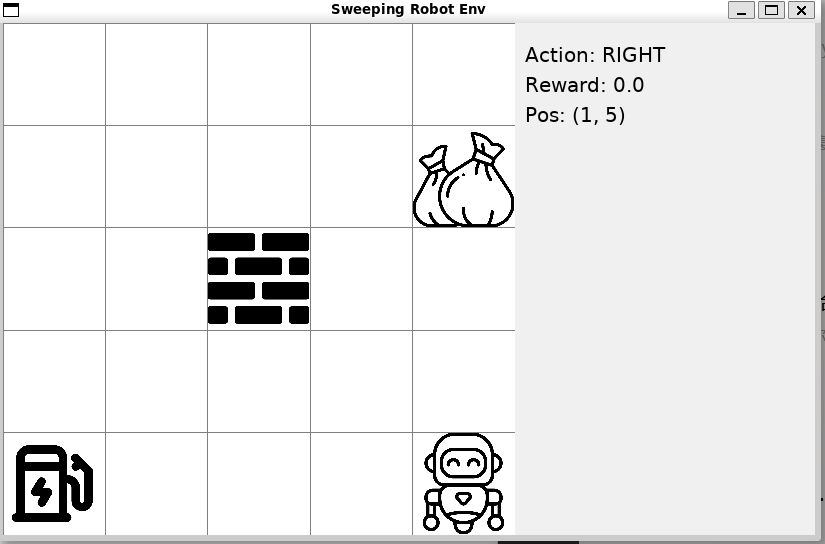
\includegraphics[width=0.48\linewidth]{figure/sweep_robot_env_render1.jpg}
% \hfill
% 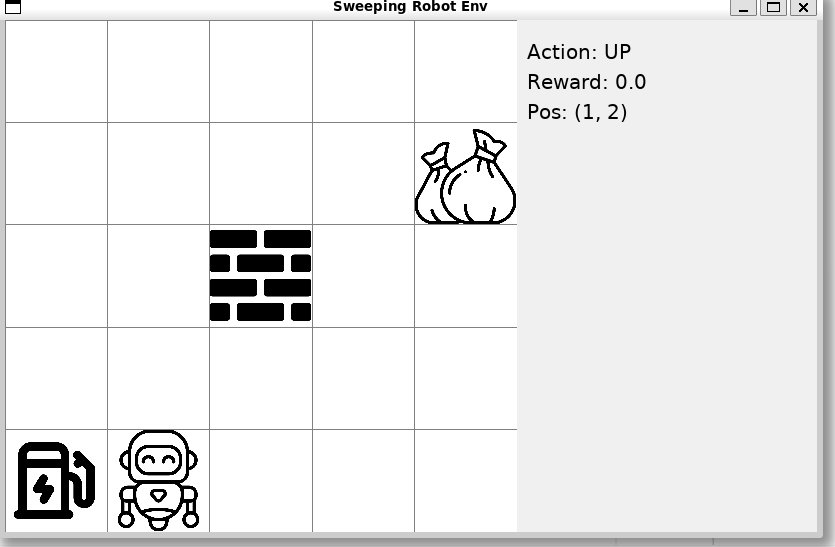
\includegraphics[width=0.48\linewidth]{figure/sweep_robot_env_render2.jpg}
% \caption{扫地机器人学习过程可视化展示(\textsf{render} 函数实现)}\label{fig:sweeping-robot-env-render}
% \end{figure}

\begin{figure}[htb]
\centering
\begin{subfigure}{0.48\linewidth}
    \centering
    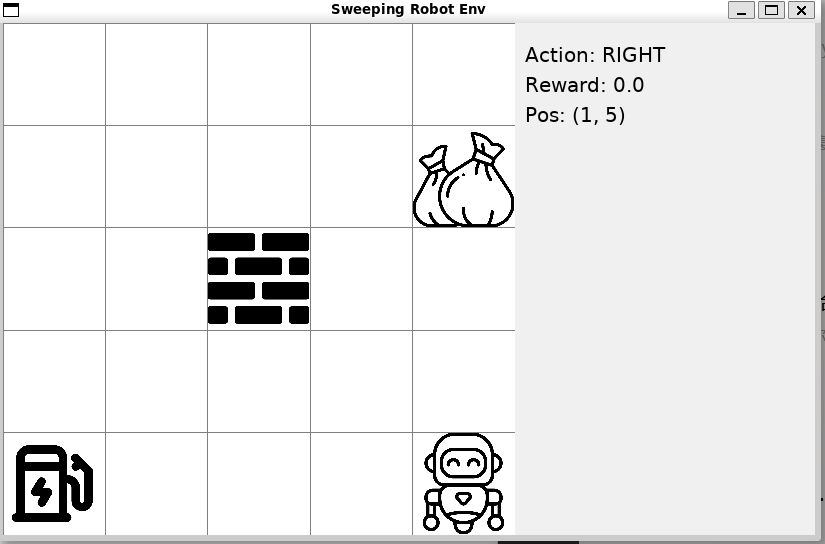
\includegraphics[width=\linewidth]{figure/sweep_robot_env_render1.jpg}
\end{subfigure}
\hfill
\begin{subfigure}{0.48\linewidth}
    \centering
    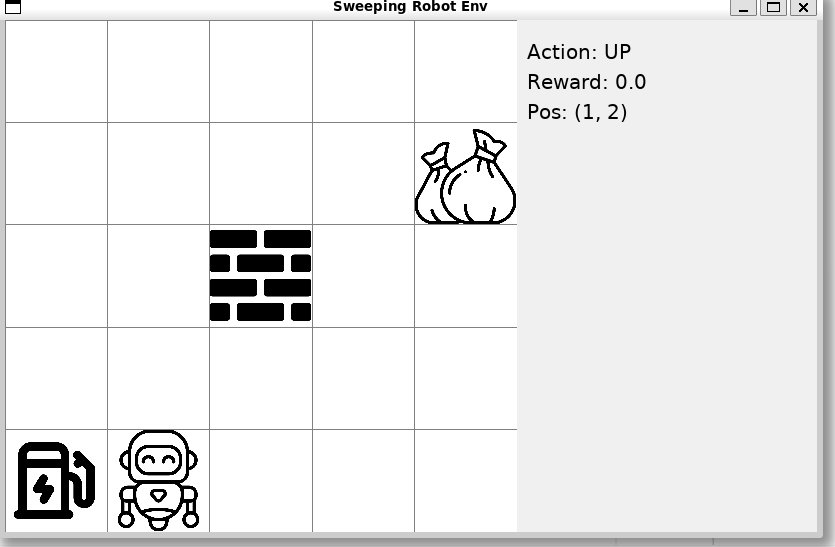
\includegraphics[width=\linewidth]{figure/sweep_robot_env_render2.jpg}
\end{subfigure}
\caption{扫地机器人学习过程可视化展示(\textsf{render} 函数实现)}
\label{fig:sweeping-robot-env-render}
\end{figure}

\subsection{具体代码}

对于扫地机器人的环境的具体代码,请参考附录~\ref{sec:sweeping-robot-env}

\section{多开关匹配}

多开关匹配是我发明的一个简单的强化学习环境,其主要的环境描写如下:

\begin{definition*}{环境描述}
\# 问题描述

    设计一个多开关匹配的强化学习环境。在该环境中,智能体的任务是通过一系列操作将开关的状态调整到目标状态。每个开关有两个可能的状态:开 (\(1\)) 或关 (\(0\))。智能体可以独立地控制每个开关的状态,置 \(1\) 代表拨动开关,置 \(0\) 代表不对开关进行操作。智能体的目标是通过最少的步骤将所有开关的状态与目标状态一致。
\end{definition*}

\subsection{使用 \textsf{spaces.MultiBinary} 构建组合构建的观测空间和动作空间}

对于这个环境,假设我们需要同时操作 \(3\) 个动作,我们需要注意的是如何构建多个动作空间构成的环境。
在这里,我们直接使用 \textsf{spaces.MultiBinary},并且官方给了一个例子。
\begin{minted}[fontsize=\small, breaklines]{python}
>>> from gymnasium.spaces import MultiBinary
>>> observation_space = MultiBinary(5, seed=42)
>>> observation_space.sample()
>>> array([1, 0, 1, 0, 1], dtype=int8)
>>> observation_space = MultiBinary([3, 2], seed=42)
>>> observation_space.sample()
>>> array([[1, 0],
           [1, 0],
           [1, 1]], dtype=int8)
\end{minted}
我们只要通过其中一个参数的大小,就可以控制这个二进制空间了。
假定我们的开关一共有 \texttt{num\_switches} 个,所以:
\begin{minted}[fontsize=\small, breaklines]{python}
self.observation_space = spaces.MultiBinary(num_switches)
self.action_space = spaces.MultiBinary(num_switches)
\end{minted}
并且通过随机设置一个目标状态,来构建我们的目标:
\begin{minted}[fontsize=\small, breaklines]{python}
self.target_state = np.random.randint(0, 2, size=num_switches)
\end{minted}
对于动作,通过 \(1\) 表示拨动开关,\(0\) 表示不拨动开关,这个在 \textsf{step} 函数中的核心逻辑为:
\begin{minted}[fontsize=\small, breaklines]{python}
self.target_state = np.random.randint(0, 2, size=num_switches)
self.state = (self.state + action) % 2
\end{minted}

\subsection{可视化展示}

我们的环境也做了一个简单的可视化(如图~\ref{fig:multiswitch-env-render}),具体代码实现需要参考代码中的 \textsf{render} 函数。

\begin{figure}[htbp]
    \centering
    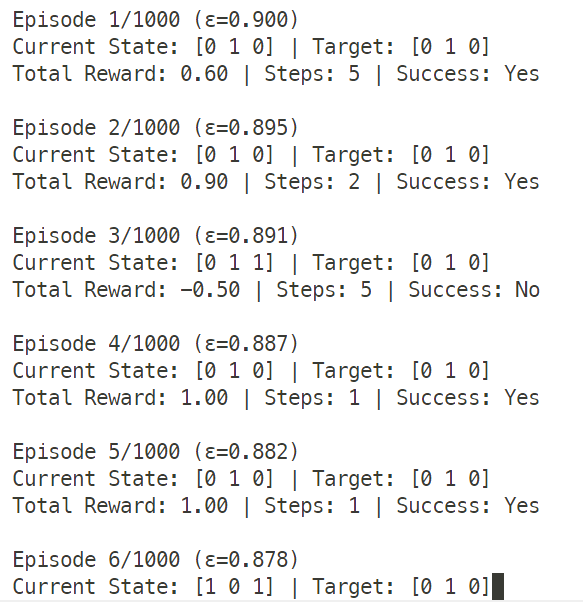
\includegraphics[width=0.5\textwidth]{figure/multi-switch-env_render1.jpg}
    \caption{扫地机器人学习过程可视化展示(\textsf{render} 函数实现)}\label{fig:multiswitch-env-render}
\end{figure}

\subsection{实现代码}

对于多开关匹配的环境的具体代码,请参考附录~\ref{sec:multi-switch-env}。

\section{Double Mountain Car}

对于我创建的 Double Mountain Car 环境,是仿造经典的离散动作版本的 MountainCar 问题的扩展版本,具体代码可以参考 \href{https://gymnasium.farama.org/environments/classic_control/mountain_car}{https://gymnasium.farama.org/environments/classic\_control/mountain\_car}。
其环境的详细描述如下:

\begin{definition*}{环境描述}
\# 问题描述

    设计一个包含 两个山地车 的强化学习环境。该环境是经典离散动作的 MountainCar 问题的扩展版本~\footnote{如果你不熟悉 MountainCar 问题,请参考 \href{https://gymnasium.farama.org/environments/classic_control/mountain_car}{https://gymnasium.farama.org/environments/classic\_control/mountain\_car}。},两个智能体(小车)必须协作,利用加速度在重力势能影响下成功爬坡,到达目标位置。两个小车可以分别独立控制,它们的任务是同时达到终点位置的目标状态,回合才会终止。这个问题与 MountainCar 问题几乎一致,但是可以帮助大家熟悉 gymnasium 库中的 \href{https://gymnasium.farama.org/api/spaces/fundamental/#gymnasium.spaces.Box}{spaces.Box} 和 \href{https://gymnasium.farama.org/api/spaces/fundamental/#gymnasium.spaces.MultiDiscrete}{spaces.MultiDiscrete} 这两个基础空间类。

\# 具体要求

对于这个问题的相关具体要求,可以仔细阅读并参考 MountainCar 问题的源代码 \href{https://github.com/Farama-Foundation/Gymnasium/blob/main/gymnasium/envs/classic_control/mountain_car.py}{gymnasium/envs/classic\_control/mountain\_car.py}。
我们唯一需要做的事情就是将原本单个 Car 的状态空间与动作空间变成 两个 Car 的状态与动作空间。
熟悉相关基础类,并初步入门多智能体控制。
\end{definition*}

在此基础上,我舍弃了使用 \textsf{render} 进行可视化,而是使用 \textsf{spaces.Box} 构建小车的观测环境和使用 \href{https://gymnasium.farama.org/api/spaces/fundamental/#gymnasium.spaces.MultiDiscrete}{\textsf{spaces.MultiDiscrete}} 来构建里两个小车的联合动作。
对于 \textsf{spaces.MultiDiscrete} 的使用,与 \textsf{spaces.MultiBinary} 类似,只是参数变成了 \textsf{np.array}。
例如对于任天堂游戏手柄,可以离散化成 \(3\) 个离散的动作空间:
\begin{itemize}
    \item 方向键:\(5\) 个离散的元素 - NOOP [0]、上 [1]、右 [2]、下 [3]、左 [4] - 参数:最小值:\(0\),最大值:\(4\)。
    \item 按钮 A:\(2\) 个离散的元素 - NOOP [0],按下 [1] - 参数:最小值:\(0\),最大值:\(1\)。
    \item 按钮 B:\(2\) 个离散的元素 - NOOP [0],按下 [1] - 参数:最小值:\(0\),最大值:\(1\)。
\end{itemize}
对应的空间代码为
\begin{minted}[fontsize=\small, breaklines]{python}
spaces.MultiDiscrete([ 5, 2, 2 ])
\end{minted}


而在我们的环境中,对应的是两个小车,各 \(3\) 个动作,而环境可以被视为一个简单的 \(4\)-维的 \textsf{spaces.Box}~\footnote{也可以通过 \textsf{spaces.Tuple} 和 \textsf{spaces.Box} 组合构建。} 所以动作和环境的初始化如下:
\begin{minted}[fontsize=\small, breaklines]{python}

...
# State bounds for both cars
self.low = np.array(
    [
        self.min_position,
        -self.max_speed,  # Car 1
        self.min_position,
        -self.max_speed,  # Car 2
    ],
    dtype=np.float32,
)

self.high = np.array(
    [
        self.max_position,
        self.max_speed,  # Car 1
        self.max_position,
        self.max_speed,  # Car 2
    ],
    dtype=np.float32,
)
...
self.action_space = spaces.MultiDiscrete([3, 3])
self.observation_space = spaces.Box(self.low, self.high, dtype=np.float32)
...
\end{minted}
其他设置都和原始的 MountainCar 问题一致。
而对于可视化操作,这里就没有实现。

\subsection{实现代码}

对于 Double Mountain Car 问题的环境的具体代码,请参考附录~\ref{sec:double-mountain-car-env}。


\chapter{实验过程及结果}

在这一部分展示强化学习算法的实现。

\section{SARAS}

我们对于扫地机器人问题,首先实现了 SARSA (State-Action-Reward-State-Action) 算法。
SARSA 是一种基于时间差分(Temporal Difference, TD)的强化学习算法,用于在智能体与环境交互过程中,学习一个状态-动作价值函数(\(Q\) 函数)。它是一个 \textbf{on-policy(依策略)} 的算法,意味着它学习的是当前行为策略下的 \(Q\) 值。

SARSA 的名字来自它更新公式中用到的五个元素:
\begin{itemize}
    \item \(S_t\):当前状态(State)
    \item \(A_t\):当前动作(Action)
    \item \(R_{t+1}\):执行动作后的即时奖励(Reward)
    \item \(S_{t+1}\):下一个状态(State)
    \item \(A_{t+1}\):在下一个状态选择的动作(Action)
\end{itemize}

SARSA 的基本更新公式为:
\[
    Q^{\texttt{new}} \left( s_t, a_t \right) \leftarrow  Q \left( s_t, a_t \right) + \alpha \left[ r_{t} + \gamma Q \left( s_{t+1}, a_{t+1} \right) - Q \left( s_t, a_t \right) \right]
\]
其中,\(\alpha\) 是学习率(learning rate),\(\gamma\) 是折扣因子(discount factor),衡量未来奖励的重要性。\(Q \left( S_t, A_t \right)\) 是状态-动作价值函数。
整个算法可以参考算法~\ref{ alg:sarsa}。

\begin{algorithm}[htbp]
\caption{SARSA 算法}\label{alg:sarsa}
\KwIn{学习率 \(\alpha\),折扣因子 \(\gamma\),探索率 \(\epsilon\),训练轮数 \(E\),最大步数 \(T\)}
\KwOut{动作-状态值函数 \(Q(s,a)\)}

初始化 \(Q\) 表为全零矩阵: \(Q(s,a) = \mathbf{0}_{\left|s\right|\times\left|a\right|}\)\;

\For{\( \text{episode} = 1 \) \KwTo \( E \)}{
    初始化环境状态 \( s_0 \)\;
    使用 \(\epsilon\)-greedy 策略,根据当前策略从状态 \(s_t\) 中选择动作 \(a_t\)例如 )\;
    \While{状态 \(s_t\) 不是终止状态 \textbf{or} t < T} {
        执行动作 \(a_t\),观察奖励 \(r_t\) 和下一个状态 \(s_{t+1}\)\;
        利用 \(\epsilon\)-greedy 策略 从状态 \(s_{t+1}\) 根据当前策略选择动作 \(a_{t+1}\)(例如 )\;
         生成随机数 \(p \sim \mathcal{U}(0,1)\)\;

        \eIf{\( p < \epsilon \)}{
            以等概率从动作集合 \( \mathcal{A} \) 中随机选择一个动作 \( a \)\;
        }{
            选择具有最大动作值的动作:\\
            \[ a \leftarrow \arg\max_{a \in \mathcal{A}} Q(s, a); \]
        }
        更新 \(Q\) 表 
        \[Q \left( s_t, a_t \right) \leftarrow  Q \left( s_t, a_t \right) + \alpha \left[ r_{t} + \gamma Q \left( s_{t+1}, a_{t+1} \right) - Q \left( s_t, a_t \right) \right];\]
        
        更新状态与动作
        \[s_t \leftarrow s_{t+1}, \qquad a_t \leftarrow a_{t+1};\]
    }
}
\Return{\( Q(s,a) \)}
\end{algorithm}

\subsection{算法实现细节}

具体实现代码参考附录~\ref{sec:saras}。
此处补充关键实现流程描述:
\begin{itemize}
    \item \textbf{状态映射}:使用 \textsf{state\_to\_index} 函数将二维坐标映射到 \(Q\) 表索引;
    \item \textbf{行为选择}:采取 \(\epsilon\)-greedy 策略在探索与利用之间平衡;
    \item \textbf{SARSA 更新}:在每一步中依据当前动作与下一个动作进行 \(Q\) 值更新;
    \item \textbf{训练结束条件}:达到最大步数或进入终止状态;
    \item \textbf{结果和策略可视化}:使用 matplotlib 绘制学习曲线,展示每轮的平均奖励。并将训练完成后将最终 \(Q\) 表策略渲染为箭头图示。
\end{itemize}

\subsection{实验结果与分析}

在这部分,展示使用 SARSA 方法控制扫地机器人的实验结果,包括策略可视化和学习曲线。

\subsubsection{策略可视化}

通过 \textsf{visualize\_policy\_from\_q} 函数生成的策略图如下所示(见图~\ref{fig:sarsa_policy})。其中箭头方向表示在各状态下的最优动作,我们可以清楚的从策略图中看到智能体能够顺利收集垃圾,获得最好的收益 \(5\),而不是在某些格子处陷入局部最优(获得充电站的收益 \(1\))。

\begin{figure}[htbp] 
    \centering 
    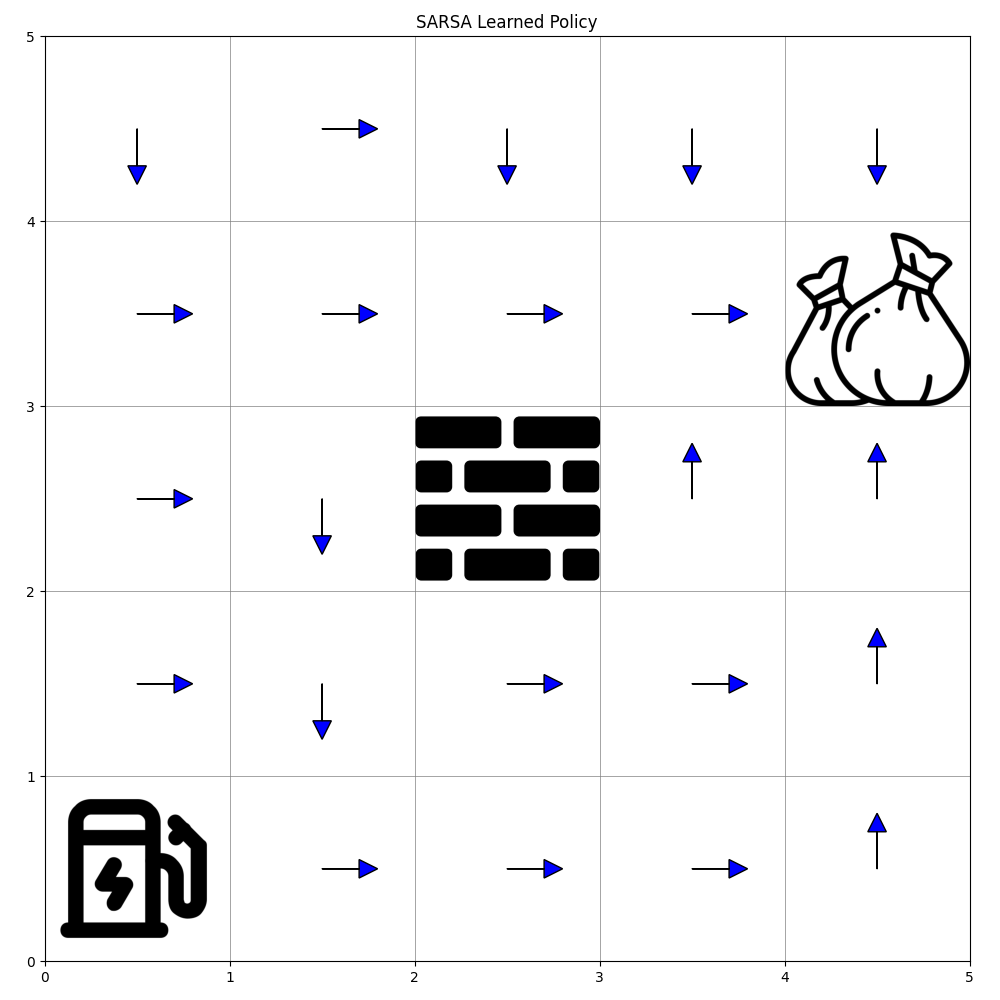
\includegraphics[width=0.5\textwidth]{figure/sweep_robot/sarsa/policy_visualization.png} 
    \caption{SARSA 策略可视化图}\label{fig:sarsa_policy} 
\end{figure}

\subsubsection{学习曲线}

训练过程中的奖励、步数与成功率变化如下图~\ref{fig:sarsa_training} 所示:
其中,我们展示了收益、步数和成功率的变化趋势。
其中我们定义成功率(Success Rate)为机器人成功达到垃圾位置而不是充电站的次数占所有试验次数的比例。
并使用了参数为 \(0.99\) 的指数移动平均值(EMA)进行展示。
可以看到,随着训练的进行,智能体的平均奖励逐渐上升,步数逐渐减少,成功率也在不断提高。这表明智能体逐渐学会了如何在环境中有效地收集垃圾而不是直接去充电站。
初期智能体尝试较多,步数波动较大;后期逐渐收敛。
我们发现成功率呈上升趋势,训练后期趋于稳定,表明智能体学会有效完成任务(捡拾垃圾而不是直接去充电站)。
一开始位置的 \(100\) \% 成功率和总步数为 \(0\) 是因为随机性导致智能体容易直接在垃圾位置附近开始,捡拾成功。

\begin{figure}[htbp] 
    \centering 
    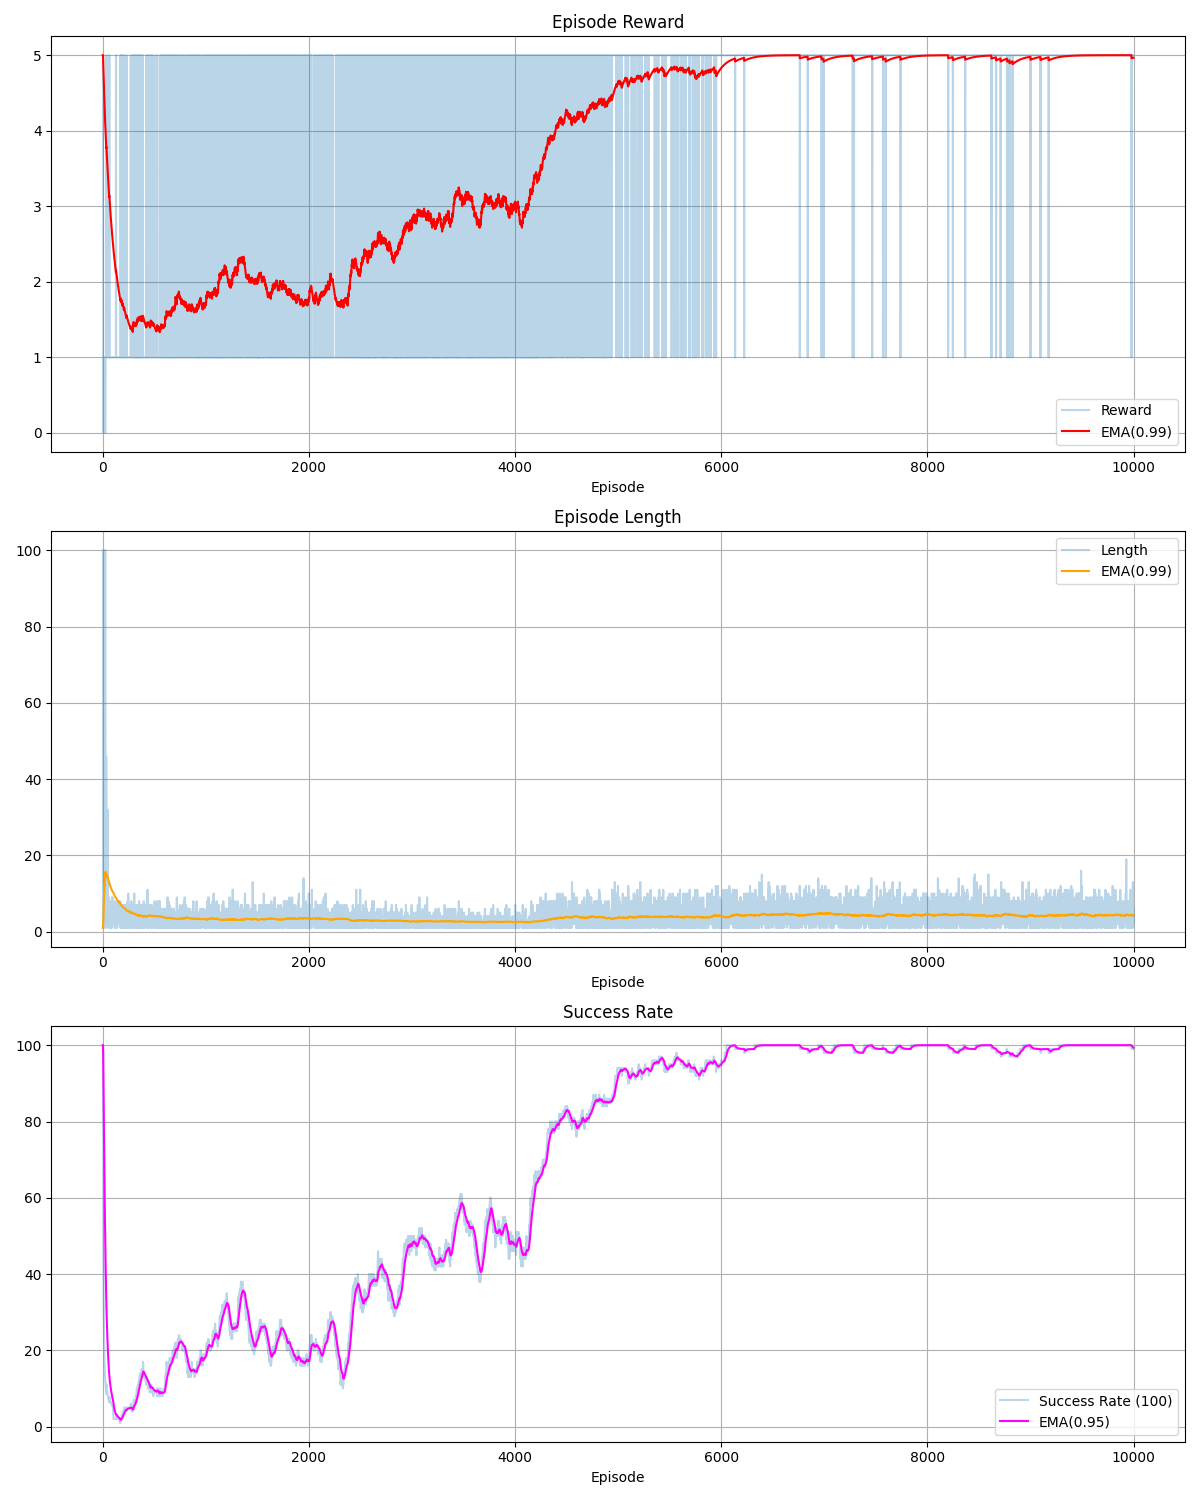
\includegraphics[width=0.8\textwidth]{figure/sweep_robot/sarsa/training_results.png} 
    \caption{SARSA 训练过程统计曲线}\label{fig:sarsa_training} 
\end{figure}

\subsection{参数设置}

本实验中的参数设置如下:
\begin{table}[htbp]
\centering
\caption{SARSA算法主要参数设置}
\label{tab:sarsa_three_line}
\begin{tabular}{ccc}
\toprule
\textbf{参数} & \textbf{取值} & \textbf{说明} \\
\midrule
\(\alpha\)(学习率) & \(0.1\) & 控制每步 \(Q\) 值更新的幅度,决定新经验对旧知识的替代程度。 \\
\(\gamma\)(折扣因子) & \(0.99\) & 衡量未来奖励对当前决策的重要性,越接近 \(1\) 表示越注重长期收益。 \\
\(\epsilon\)(探索率) & \(0.1\) & \(\epsilon\)-贪婪策略中用于随机探索的概率,平衡探索与利用。 \\
总回合数(Episodes) & \(10000\) & 智能体与环境交互的总轮数,较大值有助于收敛策略。 \\
最大步长(per episode) & \(100\) & 每回合允许的最大步数,防止陷入死循环。 \\
\bottomrule
\end{tabular}
\end{table}

\section{REINFORCE 策略梯度算法}

该实验部分采用 REINFORCE 策略梯度算法~\cite{DBLP:journals/ml/Williams92} 对清扫机器人任务进行训练。

REINFORCE 算法是一种基于策略梯度的强化学习算法,用于求解策略优化问题。
它属于无模型强化学习算法,直接通过策略来选择动作并进行优化,而不是通过值函数或环境模型来估计动作的回报。
在传统的值函数方法(如 \(Q\)-Learning 或 SARSA)中,核心目标是学习一个状态-动作值函数 \(Q \left( s, a \right)\),再通过贪婪策略派生出最优行为。

但一般认为在复杂任务中,值函数方法往往不易收敛,且对连续动作空间支持不佳。为此,引入了 \textbf{策略梯度方法(Policy Gradient Methods)},直接建模并优化一个参数化策略 \(\pi_{\theta} \left( a \mid s \right) \),以提高学习的稳定性与泛化能力。
在这一基础上,Williams et al. 提出了 REINFORCE,这也是最早的、也是最简单的一种蒙特卡洛策略梯度算法。其核心思想是:
\begin{itemize}
    \item “利用完整轨迹中的实际奖励来指导策略的改进,增强出现好结果的动作概率,抑制差结果的动作。”
\end{itemize}

策略梯度的优化目标为最大化期望总回报:
\begin{equation}\label{eq:policy_gradient_objective}
    \mathbf{J} \left( \theta \right) = \mathbb{E}_{\tau \sim \pi_{\theta}} \left[ R \left( \tau \right) \right]
\end{equation}
其中,\(\tau = \left(s_0, a_0, r_1, \dots, s_T, a_T, r_{T+1}\right)\) 表示一个完整轨迹,\(R \left( \tau \right)\) 为轨迹总回报。
通过对数概率技巧(log-derivative trick),策略梯度可以表示为:
\begin{equation}\label{eq:policy_gradient-log}
    \nabla_{\theta} \mathbf{J} \left( \theta \right) = \mathbb{E}_{\tau \sim \pi_{\theta}} \left[ \sum_{\pi_\theta} \nabla_{\theta} \log \pi_{\theta} \left( a_t \mid s_t \right) \cdot R_t \right]
\end{equation}
其中 \(R_t\) 是从时刻 \(t\) 开始的累计折扣奖励:
\[
    R_t = \sum_{k=0}^{T-t} \gamma^k r_{t+k+1}
\]
这种形式意味着——在每一步中,提高当时策略选择该动作的概率,按当前回报加权。

REINFORCE 的梯度估计是无偏的,但由于直接用回报 \(R\) 乘以 \(\log\) 概率,导致方差较大,训练不稳定。
为此,常引入 baseline(基线) 来降低方差,所以公式 (\ref{eq:policy_gradient_objective}) 可以改写为:
\begin{equation}\label{eq:policy_gradient_objective-log_baseline}
    \mathbf{J} \left( \theta \right) = \nabla_{\theta} \mathbf{J} \left( \theta \right) = \mathbb{E}_{\tau \sim \pi_{\theta}} \left[ \sum_{\pi_\theta} \nabla_{\theta} \log \pi_{\theta} \left( a_t \mid s_t \right) \cdot \left( R_t - b_t \right) \right]
\end{equation}
在本文中,我们的实现就是如公式 (\ref{eq:policy_gradient_objective-log_baseline}) 加入了 baseline 的 REINFORCE 算法。
算法归纳参考算法~\ref{agl:REINFORCE_replay},其中包含熵正则项(Entropy Regularization)来鼓励策略的探索性,算法中参数的含义和具体实现参考后文中的小节~\ref{subsubsec:REINFORCE-state-action} 部分。

\begin{algorithm}[htbp]
\caption{带经验回放的 REINFORCE 策略梯度算法}\label{agl:REINFORCE_replay}
\KwIn{策略网络 \( \pi_\theta(a \mid s) \),折扣因子 \( \gamma \),回放权重 \( \beta \),初始熵系数 \( \lambda_{\texttt{init}} \),最小熵系数 \( \lambda_{\texttt{min}} \),学习率 \( \alpha \),最大训练轮数 \( E \),经验缓存上限 \( N \),重放池大小 \(M\),最大步数 \( T \),经验回放频率 \( K \)}
\KwOut{最优策略参数 \( \theta \)}

初始化成功轨迹缓存池:\( \mathcal{M} \leftarrow \emptyset \)\;

\For{\( \text{episode} = 1 \) \KwTo \( E \)}{
    初始化环境状态 \( s_0 \)\;
    初始化轨迹存储列表:\( S \leftarrow [] \),\( A \leftarrow [] \),\( R \leftarrow [] \)\;

    \While{未终止}{
        采样动作:\( a_t \sim \pi_\theta(\cdot \mid s_t) \)\;
        执行动作,获得奖励 \( r_t \) 和新状态 \( s_{t+1} \)\;
        记录:\( S \gets S \cup \{s_t\} \),\( A \gets A \cup \{a_t\} \),\( R \gets R \cup \{r_t\} \)\;
    }

    \If{\( 成功拾取垃圾 \)}{
        将 \( (S, A, R) \) 存入成功缓存 \( \mathcal{M} \)\;
        若 \( |\mathcal{M}| > N \),则移除最旧轨迹\;
    }

    \For{\( t = 0 \) \KwTo \( T \)}{
        计算折扣回报:
        \[
        R_t \leftarrow \sum_{k=0}^{T - t} \gamma^k r_{t + k} ;
        \]
    }

    计算当前轨迹损失:
    \For{\( t = 0 \) \KwTo \( T \)}{
        \[
        \mathcal{L}_t \left( \theta \right) = -  \sum_{t=0}^{T} \left[ \hat{A}_t \log \pi_{\theta} \left( a_t \mid s_t \right) + \lambda \cdot \mathcal{H} \left( \pi_{\theta} \left( a_t \mid s_t \right) \right) \right], \quad \lambda = \max \left( \lambda_{\texttt{min}}, \lambda_{\texttt{init}} \cdot \left( 1 - \frac{e}{E} \right) \right)
        \]
    }

    \If{\( \text{episode} \bmod K = 0 \) \textbf{and} \( |\mathcal{M}| > 0 \)}{
        从 \( \mathcal{M} \) 中抽取一条成功轨迹 \( (S^{\prime}, A^{\prime}, R^{\prime}) \)\;
        重复上面步骤,计算其对应的回报 \( R^{\prime}_t \) 和损失 \( \mathcal{L}^{\prime}_t \)\;
        合并总损失:\[ \mathcal{L}_t \leftarrow \mathcal{L}_t + \beta \cdot \sum_t \mathcal{L}^{\prime}_t; \]
        \For{\( t = 0 \) \KwTo \( M \)}{
            \textbf{累加:} \( \mathcal{L}_t \leftarrow \mathcal{L}_t + \beta \cdot \mathcal{L}_t^{\prime} \)
        }
    }

    更新策略参数:
    \[
    \theta \leftarrow \theta - \alpha \nabla_\theta \sum_{t=0}^T \mathcal{L}_t
    \]
}
\Return{\( \theta \)}
\end{algorithm}


\subsection{算法实现细节}

在这一节中,我们具体展示我们代码实现的细节。具体实现代码参考附录~\ref{sec:REINFORCE}。

\subsubsection{策略网络结构设计}

策略 \(\pi_\theta \left( a \mid s\right)\) 通常用神经网络建模,输出为一个概率分布(softmax),从中采样动作。
对于此处,本实验使用一个三层全连接神经网络(\textsf{PolicyNetwork} 类)作为策略函数,输入为 one-hot 编码后的状态向量,输出为动作概率分布。网络结构如下:
\begin{itemize}
    \item 输入层:状态维度(\(5 \times 5\)网格,\(25\) 维)
    \item 两个隐藏层:各 \(64\) 个神经元
    \item 输出层:\(4\) 个动作方向(上、下、左、右)的 \texttt{Softmax} 概率
    \item 网络权重使用 Xavier 初始化,激活函数采用 ReLU,以确保训练稳定性。
\end{itemize}
具体函数如下:
\begin{minted}[fontsize=\small, breaklines]{python}
class PolicyNetwork(nn.Module):
    def __init__(self, input_size, hidden_size, output_size):
        super(PolicyNetwork, self).__init__()
        self.fc1 = nn.Linear(input_size, hidden_size)
        self.fc2 = nn.Linear(hidden_size, hidden_size)
        self.fc3 = nn.Linear(hidden_size, output_size)

        # 初始化权重
        nn.init.xavier_uniform_(self.fc1.weight)
        nn.init.xavier_uniform_(self.fc2.weight)
        nn.init.xavier_uniform_(self.fc3.weight)

        nn.init.zeros_(self.fc1.bias)
        nn.init.zeros_(self.fc2.bias)
        nn.init.zeros_(self.fc3.bias)

    def forward(self, x):
        x = F.relu(self.fc1(x))
        x = F.relu(self.fc2(x))
        x = self.fc3(x)
        # 添加数值稳定性
        # x = torch.clamp(x, min=-10, max=10)  # 防止过大的 logits
        return F.softmax(x, dim=-1)
\end{minted}

\subsubsection{状态表示与动作采样}\label{subsubsec:REINFORCE-state-action}

状态通过 \textsf{state\_to\_tensor()} 函数转换为 one-hot 编码张量,输入策略网络后返回 \texttt{Softmax} 输出作为动作概率。
通过 \textsf{torch.distributions.Categorical} 分布进行动作采样,以保持策略的随机性和探索能力。

\begin{minted}[fontsize=\small, breaklines]{python}
...
def state_to_tensor(state, size):
    """将状态转换为 one-hot 编码的张量"""
    row, col = state
    state_vector = torch.zeros(size * size)
    state_vector[row * size + col] = 1
    return state_vector
...
# 采样动作
m = Categorical(action_probs)
...
\end{minted}

\subsection{回报计算与损失函数设计}

使用 \textsf{compute\_returns()} 函数计算每一步的折扣回报:
\[
    R_t = \sum_{k=0}^{T-t} \gamma^k r_{t+k+1}
\]

为减小训练不稳定性,引入 baseline(平均回报)并标准化优势函数:

\[
    A_t = R_t - \bar{R}, \qquad \hat{A}_t = \frac{A_t - \mathbb{E}[A_t]}{\sqrt{\text{Var}(A_t)} + \varepsilon}
\]
其中 \(\mathbb{E}[A_t]\) 是优势函数 \(A\) 的均值,\(\text{Var}(A_t)\) 是方差,\(\varepsilon\) 是一个小常数(如 \(1e-8\))以避免除零错误。
并且我们引入了熵正则项(Entropy Regularization):在策略梯度方法(尤其是 REINFORCE)中,智能体在训练早期往往面临策略收敛过快、陷入局部最优的问题。为缓解这一现象,常引入熵正则项(Entropy Regularization)来鼓励策略的随机性和探索性。
熵是衡量概率分布不确定性的度量。在策略网络中,若某一时刻的动作概率分布越平均,其熵越高,说明策略具有更强的探索能力;反之,若某一动作概率接近 \(1\),则熵趋于 \(0\),表示策略已趋于确定性,可能导致提前陷入“贪婪”。
对于策略 \( \pi_{\theta} \left( a \mid s \right) \) 的动作分布,其熵定义为:
\begin{equation}
    \mathcal{H} \left( \pi_{\theta} \left( a \mid s \right) \right) = - \sum_a \pi_{\theta} \left( a \mid s \right) \log \pi_{\theta} \left( a \mid s \right)
\end{equation}
熵越大,说明动作分布越均匀,策略越具有“探索性”。
在策略优化中,我们将熵项作为额外奖励项添加至原始损失函数中,从而形成如下形式的目标函数,得到最终损失为:
\begin{equation}
    \mathcal{L} \left( \theta \right) = - \mathbb{E}_{\tau \sim \pi_{\theta}} \left[ \sum_{t=0}^{T} \hat{A}_t \log \pi_{\theta} \left( a_t \mid s_t \right) + \lambda \cdot \mathcal{H} \left( \pi_{\theta} \left( a_t \mid s_t \right) \right) \right]
\end{equation}
其中 \(\lambda\) 为熵正则项的权重系数,并会动态调整:
\[
    \lambda = \max \left( \lambda_{\texttt{min}}, \lambda_{\texttt{init}} \cdot \left( 1 - \frac{e}{E} \right) \right)
\]
其中,\(e\) 为当前训练的 episode 编号;\(E\) 为总训练轮数(即 episodes);\(\lambda_{\texttt{min}}\) 为初始熵系数(代码中为 \(0.8\));\(\lambda_{\texttt{init}}\) 为最小熵系数(代码中为 \(0.1\));早期训练阶段 \(\frac{e}{E} \approx 0 \Rightarrow \lambda \approx 0.8\),鼓励探索。训练中期至后期 \(\frac{e}{E} \approx 1 \Rightarrow \lambda \to 0.1\),逐步转向稳定策略。

代码中,熵正则项的实现如下:
\begin{minted}[fontsize=\small, breaklines]{python}
...
entropy_coef = max(0.1, 0.8 * (1 - episode / episodes))
...
entropy_bonus += m.entropy() * entropy_coef
...
loss = torch.stack(policy_loss).sum() - entropy_bonus
...
\end{minted}

\subsection{学习率调度与稳定机制}

\subsubsection{学习率调度}

实验中,优化器采用 \texttt{Adam},初始学习率为 \(0.001\),并通过 StepLR 每 \(1000\) 轮衰减至 \(95\)\%。
同时为防止梯度爆炸,引入梯度裁剪(最大范数为 \(5.0\))。此外,在每 \(50\) 轮训练中使用一次经验回放,利用之前成功轨迹进一步强化学习。

\subsubsection{经验回放机制}

在训练过程中,智能体通过与环境交互收集状态、动作、奖励等信息,并将这些信息存储在经验回放缓冲区中。
依赖于这些存储信息,我实现了\textbf{“成功经验回收机制”} 以完善训练:只保存过去成功到达目标(即成功回收垃圾)的完整轨迹,保留最近 \(10\) 条;每 \(50\) 轮训练时,从这些轨迹中随机挑选一条,加入当前训练 loss 中一同反向传播。

\rcomment[什么是“经验回收机制”?]{在强化学习中,\textbf{经验回放(Experience Replay)}指的是将过去的一些经验(即状态、动作、奖励等轨迹)保存下来,在后续训练中反复使用,而不是每次都只依赖当前的样本。}

保存成功轨迹部分代码如下:

\begin{minted}[fontsize=\small, breaklines]{python}
if total_reward >= 5:
    success_count += 1
    recent_successes.append({
        "states": states.copy(),
        "actions": actions.copy(),
        "rewards": rewards.copy()
    })
    if len(recent_successes) > 10:
        recent_successes.pop(0)
\end{minted}

每隔 \(50\) 轮回放一次

\begin{minted}[fontsize=\small, breaklines]{python}
if len(recent_successes) > 0 and episode % 50 == 0:
    success_traj = recent_successes[np.random.randint(len(recent_successes))]
    ...
    for state, action, advantage in zip(...):
        ...
        policy_loss.append(-m.log_prob(action) * advantage * 0.5)
\end{minted}

\subsection{参数设置}

本实验的参数设置可参考表~\ref{tab:reinforce-params}。

\begin{table}[htbp]
\centering
\caption{REINFORCE算法实验参数设置}
\label{tab:reinforce-params}
\begin{tabular}{@{}lll@{}}
\toprule
\textbf{参数名称} & \textbf{含义} & \textbf{设置值} \\
\midrule
Grid Size & 环境网格大小 & \( 5 \times 5 \) \\
Input Size & 状态维度(One-hot 编码) & \( 25 \) \\
Hidden Size & 隐藏层神经元数 & \( 64 \) \\
Output Size & 动作空间维度(上下左右) & \( 4 \) \\
Learning Rate & 学习率 & \( 0.001 \) \\
Optimizer & 优化器类型 & Adam \\
Discount Factor \(\gamma\) & 折扣因子 & \( 0.995 \) \\
Entropy Coefficient \(\lambda\) & 熵正则化系数 & \( 0.8 \rightarrow 0.1 \)(线性递减) \\
Gradient Clipping & 梯度裁剪最大范数 & \( 5.0 \) \\
Scheduler & 学习率调度器 & StepLR,每 \( 1000 \) 轮乘 \( 0.95 \) \\
Episodes & 总训练轮数 & \( 10000 \) \\
Max Steps / Episode & 每回合最大步数 & 动态增长,\( 50 \rightarrow 100 \) \\
EMA Smoothing Factor & EMA 平滑系数(奖励/步数) & \( 0.95 \sim 0.99 \) \\
Replay Frequency & 成功轨迹经验回放频率 & 每 \( 50 \) 轮一次 \\
Replay Buffer Size & 成功轨迹最大存储数量 & \( 10 \) 条 \\
Replay Weight & 成功轨迹回放权重 & \( 0.5 \) \\
\bottomrule
\end{tabular}
\end{table}

\subsubsection{实验结果与分析}

\subsubsection{策略可视化}

通过 \textsf{visualize\_policy} 函数生成的策略图如下所示(见图~\ref{fig:REINFORCE_policy})。其中箭头方向表示在各位置动作策略(只绘制概率 \(> 0.1\) 的策略。

\begin{figure}[htbp] 
    \centering 
    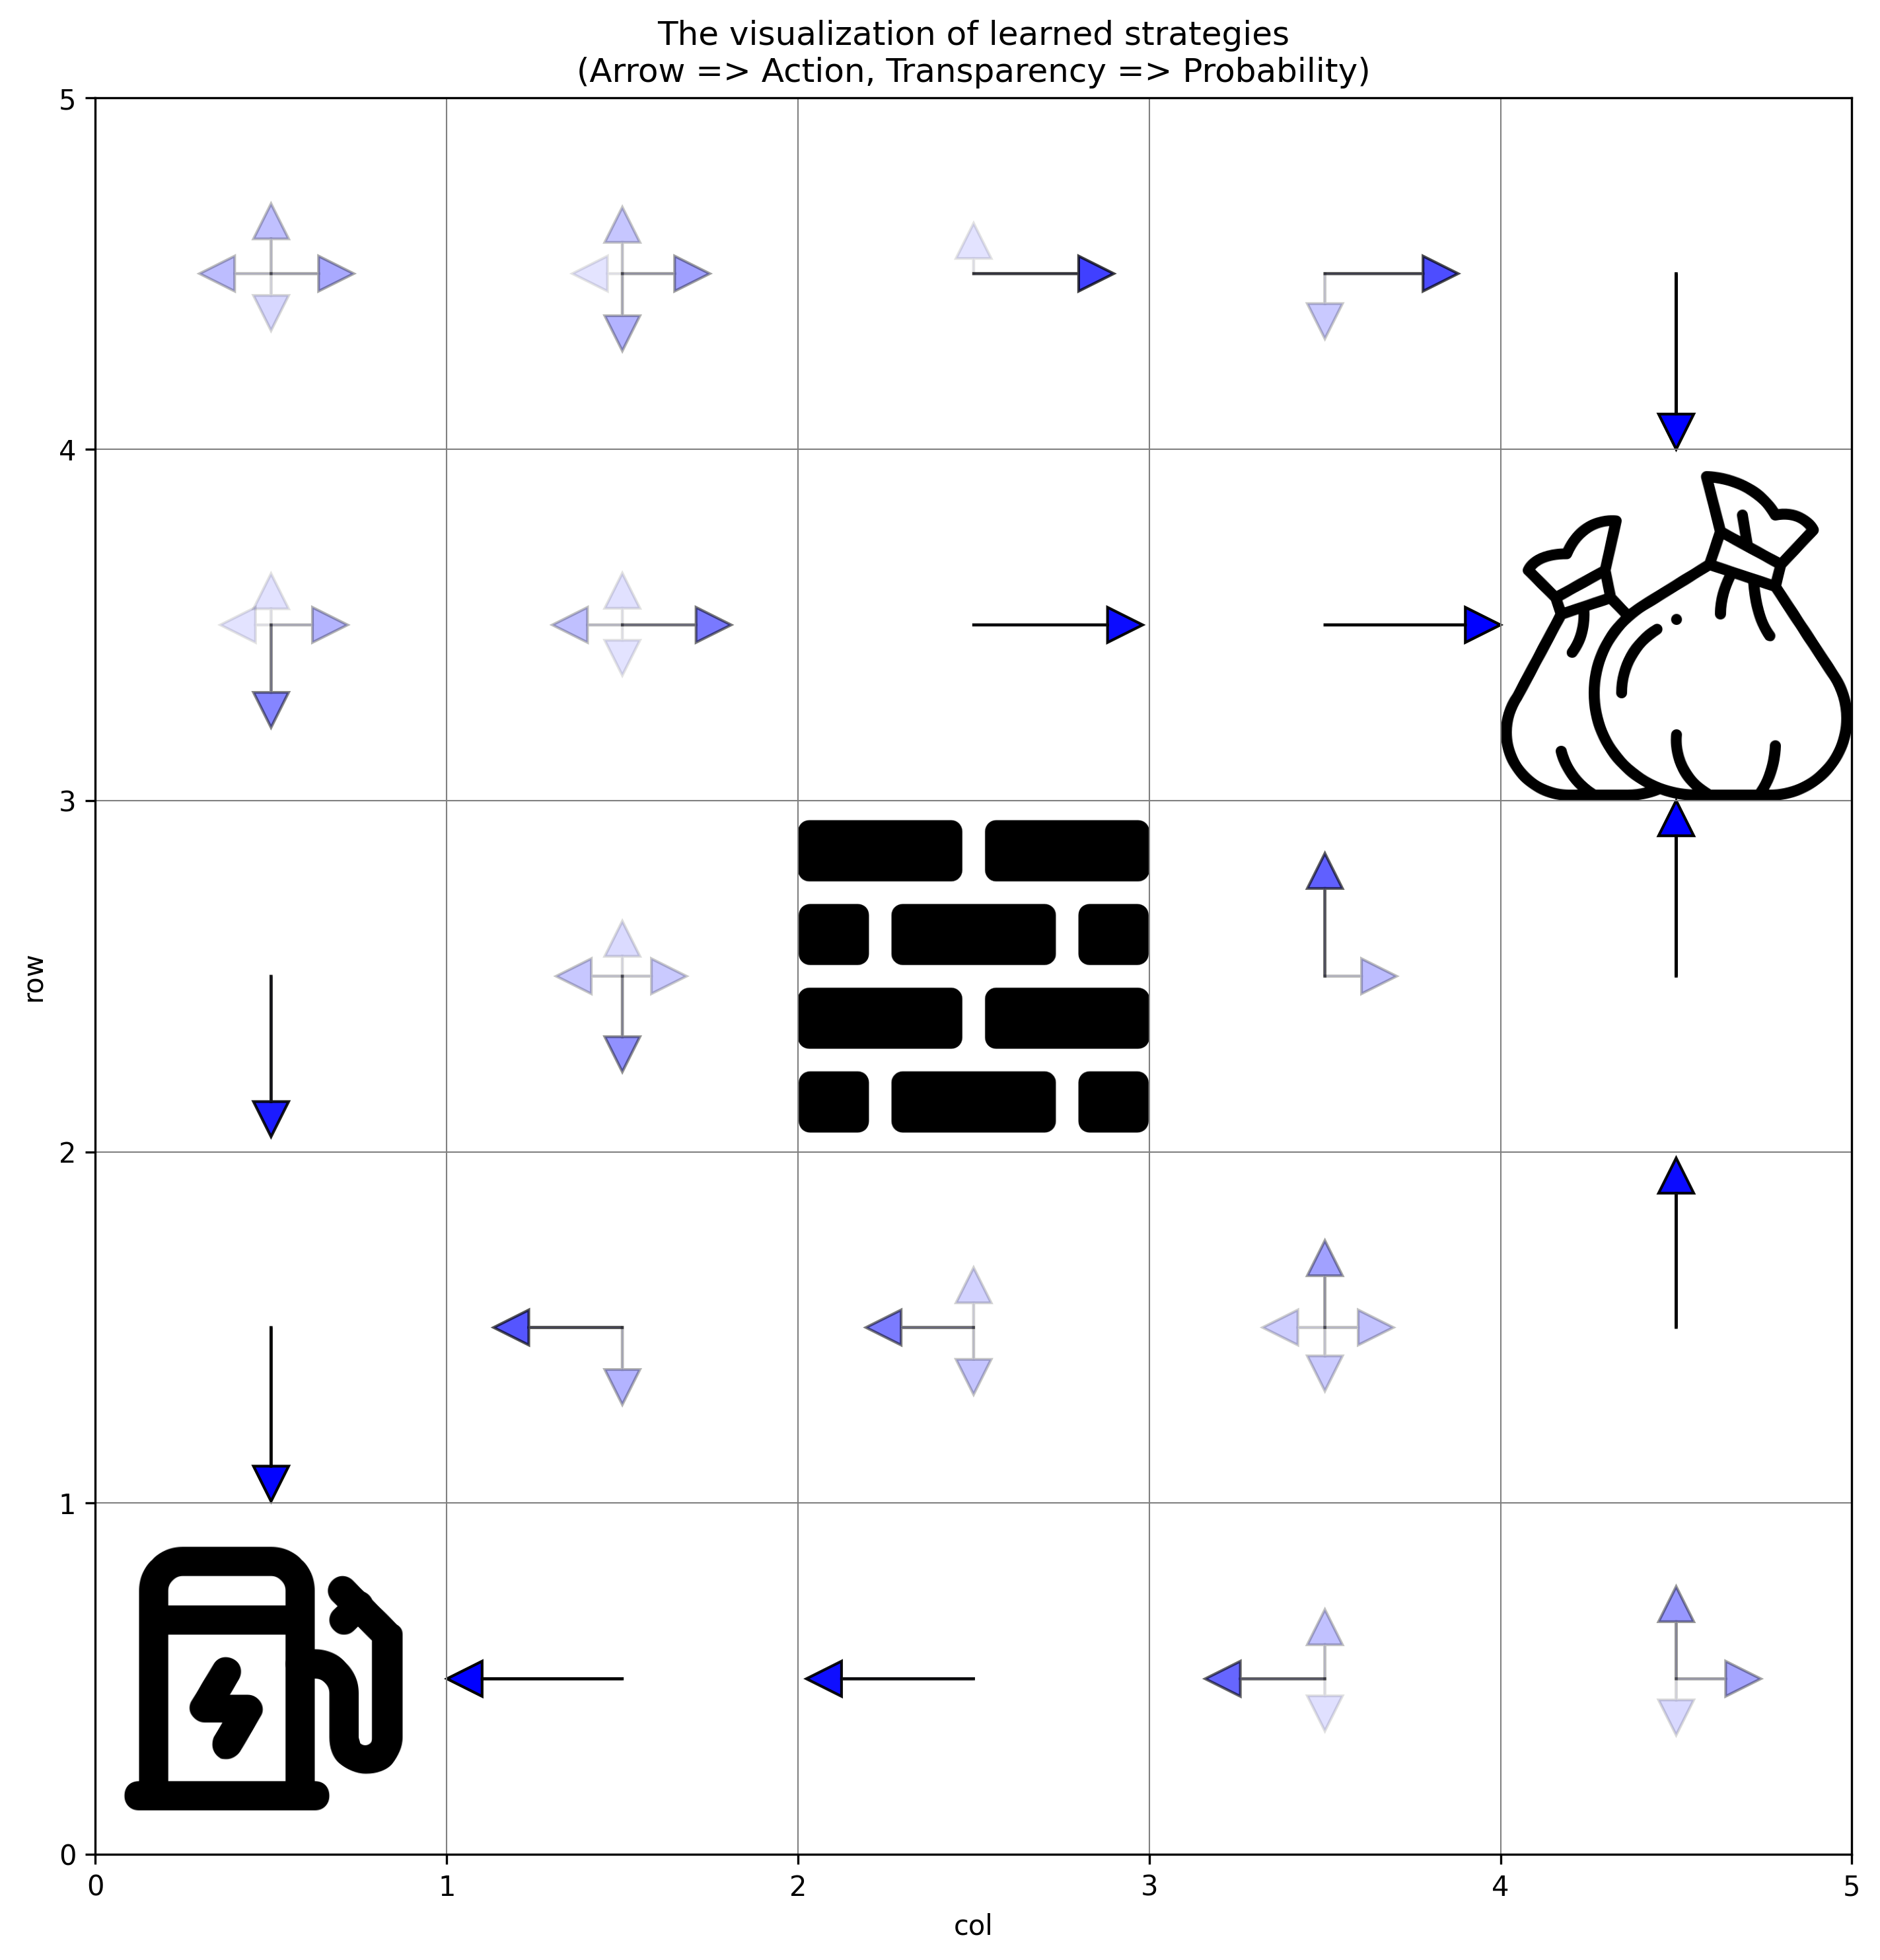
\includegraphics[width=0.5\textwidth]{figure/sweep_robot/REINFORCE/policy_visualization.png} 
    \caption{REINFORCE 策略梯度算法的策略可视化图}\label{fig:REINFORCE_policy} 
\end{figure}

\subsubsection{学习曲线}

本实验的学习曲线如图~\ref{fig:REINFORCE_training} 所示。我们展示了收益、步数和成功率的变化趋势。

\begin{figure}[htbp] 
    \centering 
    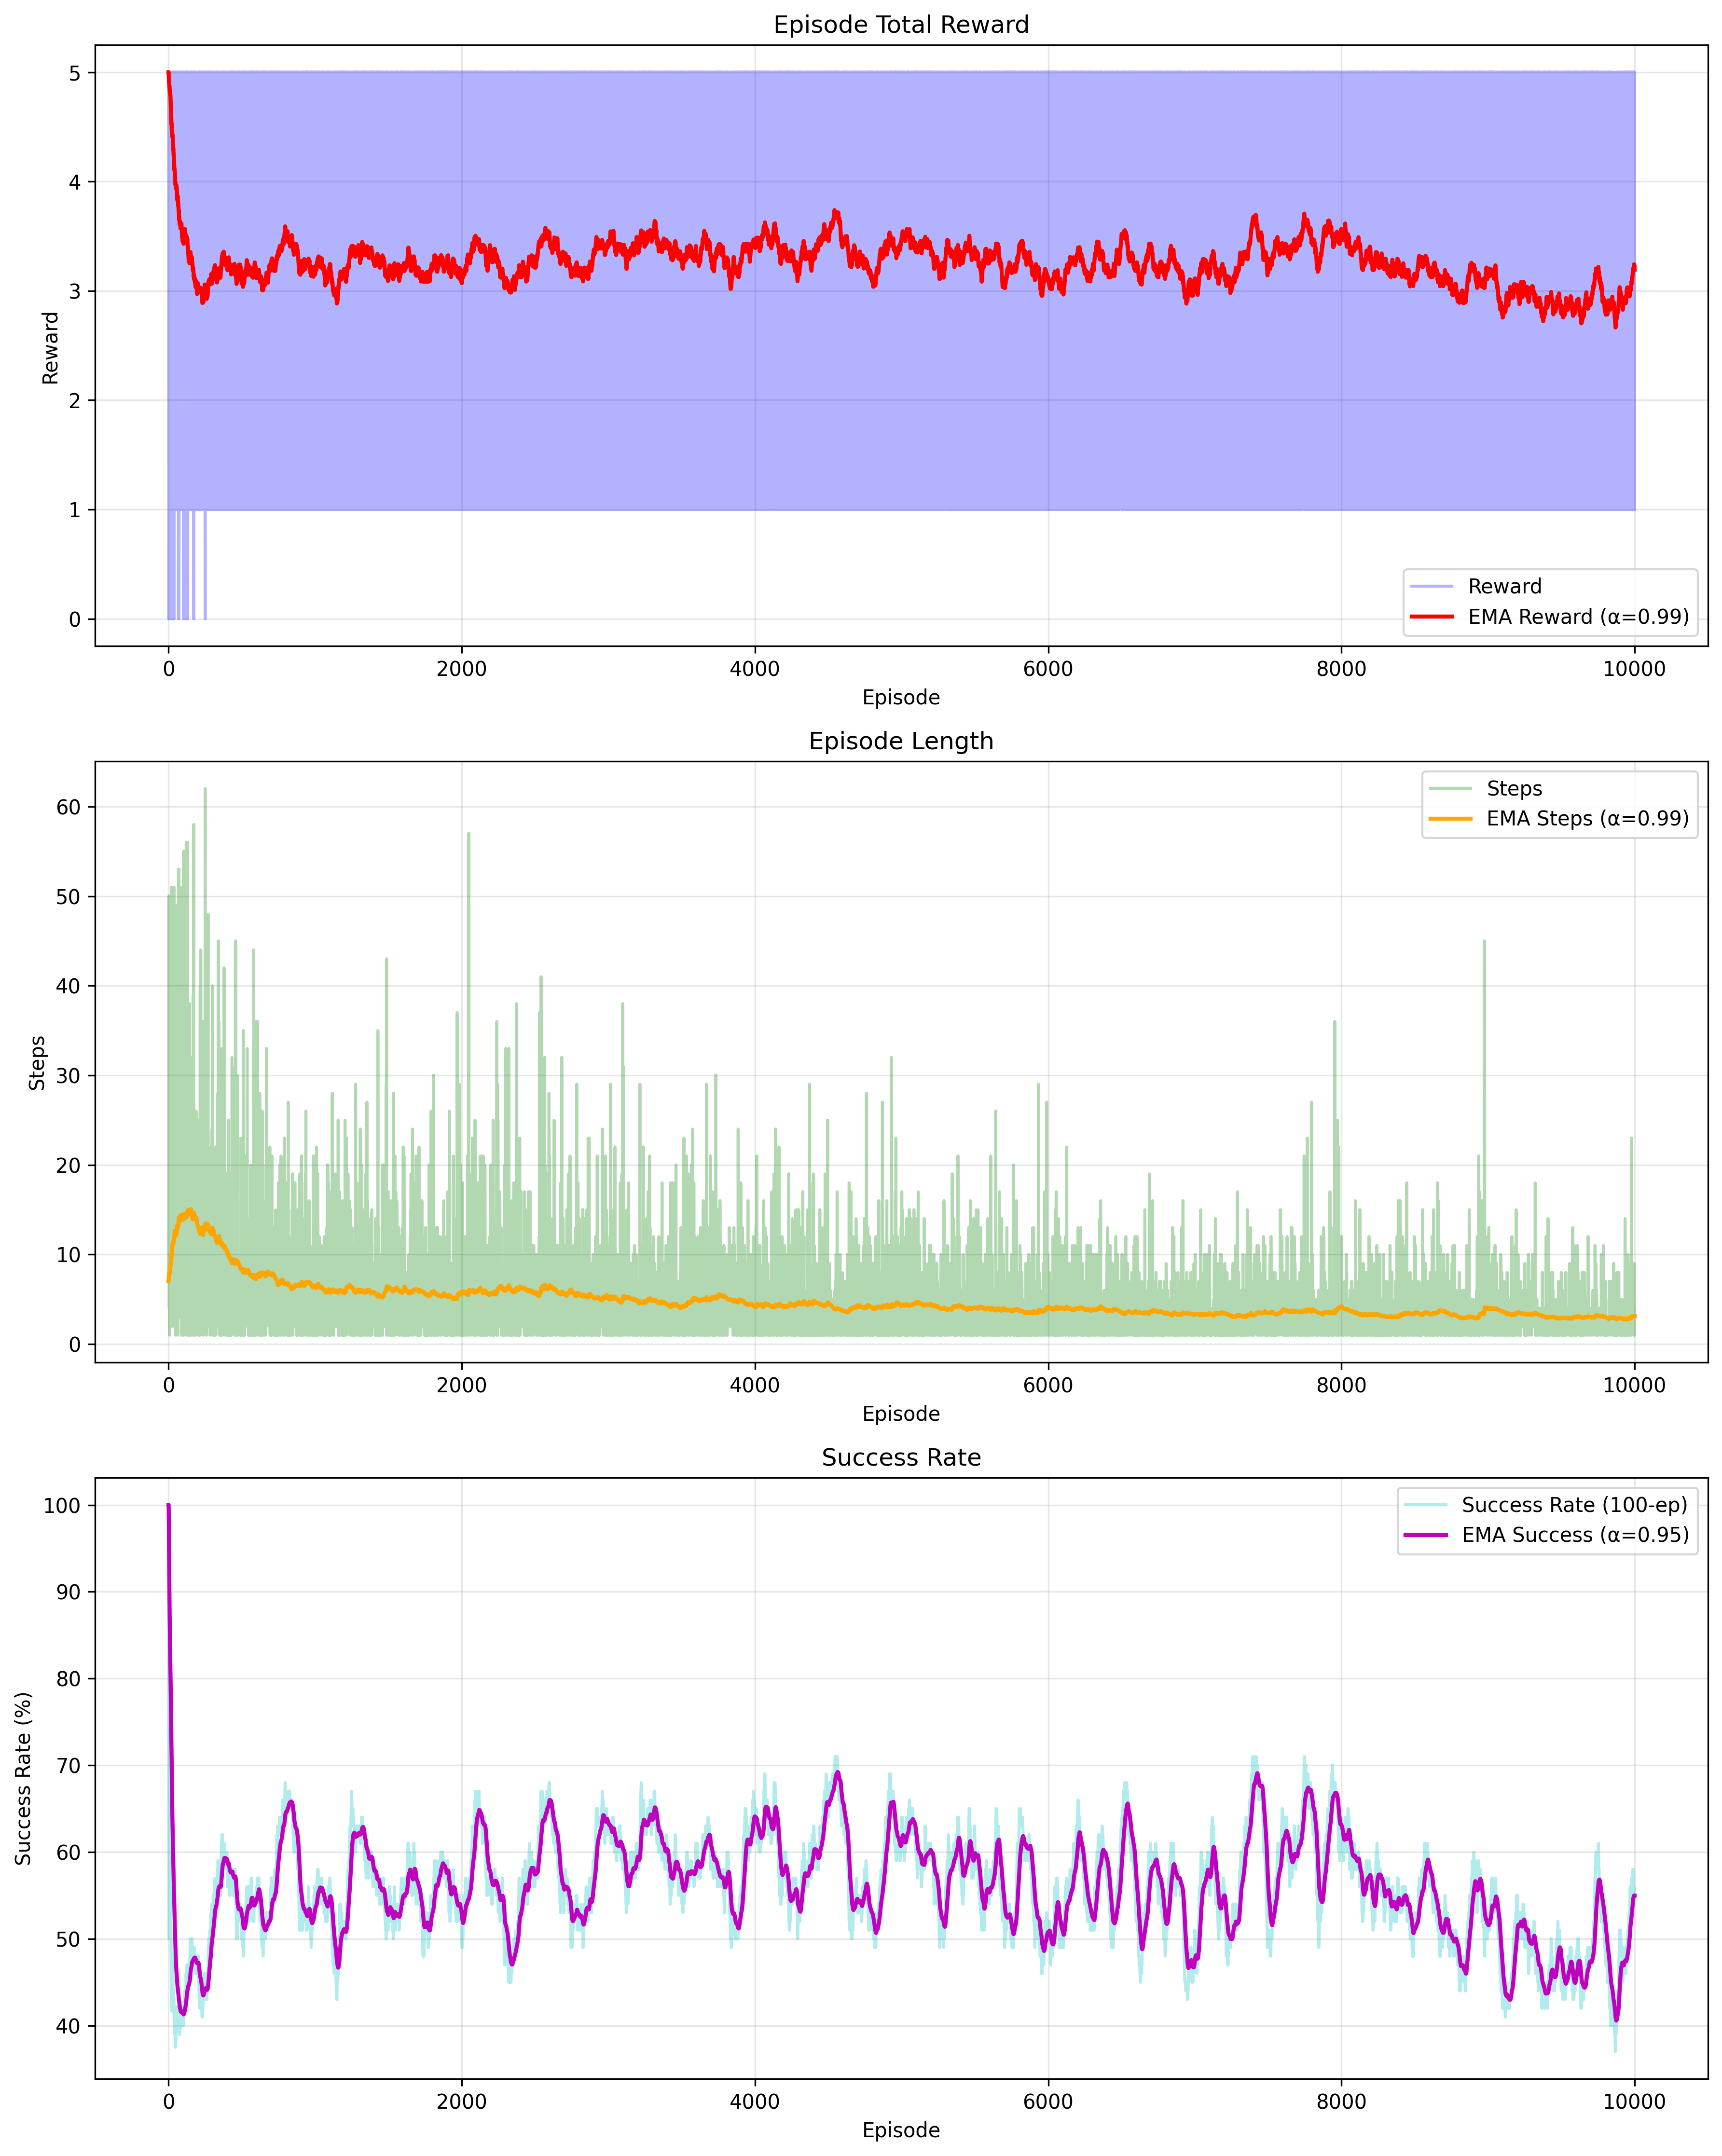
\includegraphics[width=0.8\textwidth]{figure/sweep_robot/REINFORCE/training_results.png} 
    \caption{REINFORCE 策略梯度算法的策略可视化图}\label{fig:REINFORCE_training} 
\end{figure}

可以发现,REINFORCE 算法在训练过程中,平均奖励水平较低,且波动较大。智能体在充电站附近停留时间过长,导致平均奖励水平未能有效提升,对于 SARAS 算法的表现较差。

\subsubsection{总结}

分析表明,REINFORCE 策略梯度算法在当前环境下未能习得有效的策略。
尽管智能体在训练过程中能够逐步收集垃圾,但其在充电站停留时间过长,导致平均奖励水平较低。
如图~\ref{fig:REINFORCE_policy} 所示,机器人越接近充电站,其选择充电而非收集垃圾的倾向越明显,这表明智能体可能在学习过程中陷入了局部最优解。

究其原因,核心问题在于环境奖励的稀疏性:仅在充电桩和垃圾位置提供奖励,使得智能体难以学习最优策略。其决策严重依赖轨迹末端状态,一旦习得“快速终止回合”的行为模式,便容易形成次优策略。

此外,REINFORCE 算法固有的特性也加剧了这一问题:
\begin{itemize}
    \item 回合制更新限制:算法需等待整个回合结束后才能获得总回报。在奖励稀疏或环境复杂的情况下,这显著增加了陷入次优策略的风险。
    \item  \textbf{反馈延迟}:由于回报基于回合总奖励,中间决策的优劣无法即时反馈给智能体。智能体需待回合结束方能评估决策正确性。若关键决策发生于回合后期,将导致梯度更新延迟,阻碍策略及时修正。
    \item \textbf{稀疏奖励}:在仅终点(垃圾/充电桩)提供奖励的稀疏环境下,智能体需经历较长路径才能获得有效信息,极易因探索不足而固守次优策略。
    \item \textbf{更新噪声与不稳定性}:依赖整条轨迹回报进行全局更新,使得梯度易受随机噪声干扰,导致训练过程波动较大,难以收敛至全局最优策略。
\end{itemize}

REINFORCE 算法在这种环境下的收敛速度较慢,且容易受到高方差的影响,导致学习不稳定。

\section{\(Q\)-learning 算法}

在这部分,展示我实现的对于多开关匹配环境的智能体 \(Q\)-learning 实现代码。

\begin{minted}[frame=single, fontsize=\small, linenos, breaklines]{python}
import os
from collections import deque

import matplotlib.pyplot as plt
import numpy as np

from multi_switch_env import MultiSwitchEnv


class TrainingMonitor:
    """训练监控器,记录各种指标用于绘图"""

    def __init__(self):
        self.episode_rewards = []
        self.episode_lengths = []
        self.q_value_mean = []
        self.q_value_max = []
        self.success_rate = deque(maxlen=20)  # 滑动窗口记录最近 20 个 episode 的成功率
        self.epsilon_values = []

    def record_episode(self, total_reward, episode_length, success):
        self.episode_rewards.append(total_reward)
        self.episode_lengths.append(episode_length)
        self.success_rate.append(1.0 if success else 0.0)

    def record_q_values(self, q_table):
        self.q_value_mean.append(np.mean(q_table))
        self.q_value_max.append(np.max(q_table))

    def record_epsilon(self, epsilon):
        self.epsilon_values.append(epsilon)

    def compute_ema(self, data, alpha=0.9):
        """计算指数加权移动平均(EMA)"""
        ema = np.zeros_like(data, dtype=float)
        if len(data) > 0:
            ema[0] = data[0]
            for i in range(1, len(data)):
                ema[i] = alpha * ema[i - 1] + (1 - alpha) * data[i]
        return ema

    def plot_results(self, save_path="/multi_switch/training_results.png"):
        """绘制训练结果的综合图表"""
        fig, axes = plt.subplots(2, 3, figsize=(15, 10))
        fig.suptitle("Multi-Switch Environment Training Metrics", fontsize=16)

        # 设置统一的EMA参数
        ema_alpha = 0.95

        # 1. Episode Rewards
        ax1 = axes[0, 0]
        ax1.plot(
            self.episode_rewards,
            alpha=0.3,
            color="blue",
            linewidth=1,
            label="Raw Rewards",
        )
        # 添加EMA平滑线
        if len(self.episode_rewards) > 1:
            ema_rewards = self.compute_ema(self.episode_rewards, ema_alpha)
            ax1.plot(ema_rewards, "b-", linewidth=2.5, label=f"EMA ($\alpha$={ema_alpha})")
        ax1.set_xlabel("Episode")
        ax1.set_ylabel("Total Reward")
        ax1.set_title("Episode Rewards Over Time")
        ax1.legend()
        ax1.grid(True, alpha=0.3)

        # 2. Episode Lengths
        ax2 = axes[0, 1]
        ax2.plot(self.episode_lengths, "g-", alpha=0.3, linewidth=1, label="Raw Steps")
        if len(self.episode_lengths) > 1:
            ema_lengths = self.compute_ema(self.episode_lengths, ema_alpha)
            ax2.plot(ema_lengths, "g-", linewidth=2.5, label=f"EMA ($\alpha$={ema_alpha})")
        ax2.set_xlabel("Episode")
        ax2.set_ylabel("Steps")
        ax2.set_title("Episode Length (Steps to Complete)")
        ax2.legend()
        ax2.grid(True, alpha=0.3)

        # 3. Success Rate
        ax3 = axes[0, 2]
        if len(self.success_rate) > 0:
            success_rates = []
            for i in range(len(self.episode_rewards)):
                end_idx = min(i + 1, len(self.success_rate))
                start_idx = max(0, end_idx - 20)
                if end_idx > start_idx:
                    rate = sum(list(self.success_rate)[start_idx:end_idx]) / (
                        end_idx - start_idx
                    )
                    success_rates.append(rate * 100)
            ax3.plot(
                success_rates, "c-", alpha=0.3, linewidth=1, label="20-Episode Window"
            )
            if len(success_rates) > 1:
                ema_success = self.compute_ema(success_rates, ema_alpha)
                ax3.plot(ema_success, "b-", linewidth=2.5, label=f"EMA ($\alpha$={ema_alpha})")
        ax3.set_xlabel("Episode")
        ax3.set_ylabel("Success Rate (%)")
        ax3.set_title("Success Rate")
        ax3.legend()
        ax3.grid(True, alpha=0.3)
        ax3.set_ylim([0, 105])

        # 4. Q-Value Mean
        ax4 = axes[1, 0]
        ax4.plot(self.q_value_mean, "purple", alpha=0.3, linewidth=1, label="Raw Mean")
        if len(self.q_value_mean) > 1:
            ema_q_mean = self.compute_ema(self.q_value_mean, ema_alpha)
            ax4.plot(
                ema_q_mean, color="purple", linewidth=2.5, label=f"EMA ($\alpha$={ema_alpha})"
            )
        ax4.set_xlabel("Episode")
        ax4.set_ylabel("Mean Q-Value")
        ax4.set_title("Average Q-Value Over Time")
        ax4.legend()
        ax4.grid(True, alpha=0.3)

        # 5. Q-Value Max
        ax5 = axes[1, 1]
        ax5.plot(self.q_value_max, "orange", alpha=0.3, linewidth=1, label="Raw Max")
        if len(self.q_value_max) > 1:
            ema_q_max = self.compute_ema(self.q_value_max, ema_alpha)
            ax5.plot(
                ema_q_max, color="orange", linewidth=2.5, label=f"EMA ($\alpha$={ema_alpha})"
            )
        ax5.set_xlabel("Episode")
        ax5.set_ylabel("Max Q-Value")
        ax5.set_title("Maximum Q-Value Over Time")
        ax5.legend()
        ax5.grid(True, alpha=0.3)

        # 6. Epsilon Decay
        ax6 = axes[1, 2]
        if self.epsilon_values:
            ax6.plot(
                self.epsilon_values, "red", alpha=0.3, linewidth=1, label="Raw Epsilon"
            )
            if len(self.epsilon_values) > 1:
                ema_epsilon = self.compute_ema(self.epsilon_values, ema_alpha)
                ax6.plot(
                    ema_epsilon, "red", linewidth=2.5, label=f"EMA ($\alpha$={ema_alpha})"
                )
            ax6.set_xlabel("Episode")
            ax6.set_ylabel("Epsilon")
            ax6.set_title("Exploration Rate (Epsilon) Decay")
            ax6.legend()
            ax6.grid(True, alpha=0.3)

        plt.tight_layout()
        plt.savefig(save_path, dpi=300, bbox_inches="tight")

    def plot_q_heatmap(self, q_table, episode, save_path="q_heatmap.png"):
        """绘制Q表的热力图(仅适用于小规模Q表)"""
        # 将多维Q表展平为2D用于可视化
        flat_shape = (np.prod(q_table.shape[:3]), np.prod(q_table.shape[3:]))
        q_flat = q_table.reshape(flat_shape)

        plt.figure(figsize=(10, 8))
        plt.imshow(q_flat, cmap="coolwarm", aspect="auto")
        plt.colorbar(label="Q-Value")
        plt.title(f"Q-Table Heatmap at Episode {episode}")
        plt.xlabel("Action Combinations")
        plt.ylabel("State Combinations")
        plt.tight_layout()
        plt.savefig(save_path, dpi=300, bbox_inches="tight")
        plt.close()


def visualize_top_actions(
    q_table,
    target_state,
    num_switches=3,
    top_k=3,
    save_path="res/multi_switch/top_actions_visualization.png",
):
    """
    对于每一个可能的状态,绘制其对应Q值最高的 top_k 个动作。
    并在标题中标注目标状态。
    """
    state_space = [list(s) for s in np.ndindex(*(2,) * num_switches)]

    rows, cols = 2, 4  # 设置子图分布为 2 行 4 列
    fig, axes = plt.subplots(rows, cols, figsize=(cols * 4, rows * 4))
    axes = axes.flatten()

    for ax, state in zip(axes, state_space):
        state_idx = tuple(state)
        q_values = q_table[state_idx]

        flat_qs = q_values.reshape(-1)
        top_action_indices = flat_qs.argsort()[-top_k:][::-1]  # 降序取前k
        top_q_values = flat_qs[top_action_indices]
        top_actions = [
            np.unravel_index(idx, q_values.shape) for idx in top_action_indices
        ]

        labels = ["".join(map(str, a)) for a in top_actions]

        ax.bar(range(top_k), top_q_values)
        ax.set_xticks(range(top_k))
        ax.set_xticklabels(labels, rotation=45)
        ax.set_title(
            f"State: {''.join(map(str, state))}\nTarget: {''.join(map(str, target_state))}"
        )
        ax.set_ylabel("Q-Value")

    # 删除多余的子图
    for ax in axes[len(state_space) :]:
        ax.axis("off")

    plt.tight_layout()
    plt.suptitle("Top Actions per State", fontsize=16, y=1.05)
    plt.savefig(save_path, dpi=300, bbox_inches="tight")
    plt.close()


def create_folder(path):
    # 判断文件夹是否存在
    if not os.path.exists(path):
        # 如果文件夹不存在,则创建
        os.makedirs(path)


if __name__ == "__main__":
    create_folder("res/multi_switch")

    # 设置随机种子以便复现
    np.random.seed(42)

    env = MultiSwitchEnv(render_mode="human", num_switches=3)
    q_table = np.zeros([2] * 3 + [2] * 3)  # Q-table shape: (2,2,2,2,2,2)

    # 超参数
    alpha = 0.1  # 学习率
    gamma = 0.95  # 折扣因子
    epsilon_start = 0.9  # 初始探索率
    epsilon_end = 0.01  # 最终探索率
    epsilon_decay = 0.995  # 探索率衰减
    episodes = 1000  # 增加训练轮数以更好观察曲线

    # 创建训练监控器
    monitor = TrainingMonitor()

    # 训练循环
    epsilon = epsilon_start

    for episode in range(episodes):
        obs, _ = env.reset()
        done = False
        truncated = False
        total_reward = 0
        steps = 0

        print(f"\nEpisode {episode + 1}/{episodes} ($\epsilon$={epsilon:.3f})")

        while not done and not truncated:
            obs_idx = tuple(obs)

            # $\epsilon$-贪婪策略
            if np.random.rand() < epsilon:
                action = env.action_space.sample()
            else:
                action = np.unravel_index(
                    np.argmax(q_table[obs_idx]), q_table[obs_idx].shape
                )

            next_obs, reward, done, truncated, _ = env.step(np.array(action))
            next_obs_idx = tuple(next_obs)

            # Q-learning 更新
            best_next = np.max(q_table[next_obs_idx])
            q_table[obs_idx + tuple(action)] += alpha * (
                reward + gamma * best_next - q_table[obs_idx + tuple(action)]
            )

            obs = next_obs
            total_reward += reward
            steps += 1

            if env.render_mode == "human":
                env.render()

        # 记录训练数据
        monitor.record_episode(total_reward, steps, done)
        monitor.record_q_values(q_table)
        monitor.record_epsilon(epsilon)

        # 衰减探索率
        epsilon = max(epsilon_end, epsilon * epsilon_decay)

        print(
            f"\nTotal Reward: {total_reward:.2f} | Steps: {steps} | Success: {'Yes' if done else 'No'}"
        )

        # 每 100 个 episode 保存一次Q表热力图
        if (episode + 1) % 100 == 0:
            monitor.plot_q_heatmap(
                q_table,
                episode + 1,
                f"res/multi_switch/q_heatmap_episode_{episode + 1}.png",
            )

    env.close()

    # 绘制所有训练结果
    print("\n正在生成训练结果图表...")
    monitor.plot_results("res/multi_switch/multiswitch_training_results.png")

    # 打印最终统计信息
    print("\n=== 训练完成 ===")
    print(f"最终成功率: {np.mean(list(monitor.success_rate)) * 100:.1f}%")
    print(f"最后 10 轮平均奖励: {np.mean(monitor.episode_rewards[-10:]):.2f}")
    print(f"Q 表平均值: {np.mean(q_table):.4f}")
    print(f"Q 表最大值: {np.max(q_table):.4f}")

    # 测试训练好的策略
    print("\n=== 测试最终策略 (贪婪策略) ===")
    test_episodes = 10
    test_rewards = []

    for i in range(test_episodes):
        obs, _ = env.reset()
        done = False
        truncated = False
        total_reward = 0

        while not done and not truncated:
            obs_idx = tuple(obs)
            # 使用纯贪婪策略
            action = np.unravel_index(
                np.argmax(q_table[obs_idx]), q_table[obs_idx].shape
            )
            obs, reward, done, truncated, _ = env.step(np.array(action))
            total_reward += reward

        test_rewards.append(total_reward)
        print(
            f"测试 {i + 1}: 奖励 = {total_reward:.2f}, 成功 = {'是' if done else '否'}"
        )

    print(f"\n测试平均奖励: {np.mean(test_rewards):.2f}")
    print(f"测试成功率: {sum(r > 0 for r in test_rewards) / test_episodes * 100:.0f}%")

    visualize_top_actions(
        q_table, target_state=env.target_state, num_switches=3, top_k=3
    )

\end{minted}

\section{PPO}

本实验旨在验证 Proximal Policy Optimization(PPO)算法在多智能体协作环境——Double Mountain Car 环境中的表现。Double Mountain Car 中的两个小车需要独立控制并协作以达到各自目标位置。
本实验拟通过训练 PPO 智能体,探索其在多维动作空间下的学习效果和稳定性。

本实验基于 \href{https://github.com/DLR-RM/stable-baselines3}{Stable Baselines3} 中 PPO 实现算法实现,结合自定义的 Double Mountain Car 环境进行训练。该环境状态空间为四维向量,包含两个小车的位置与速度;动作空间为两个离散动作的组合(每个小车 \(3\) 个动作),共计 \(9\) 个联合动作。为了简化训练,使用了动作封装器将 MultiDiscrete 动作空间映射为单一离散动作空间。

具体代码实现参考附录~\ref{sec:ppo}。

\subsection{实验结果}

训练过程中,智能体不断学习如何通过两个小车的协作调整动作以最大化累计奖励。奖励设计包含每步 \(-1\) 的基础惩罚及基于两个小车位置变化的稠密奖励,促使智能体更快向目标位置移动。采用状态和奖励归一化策略,提高训练的收敛速度和稳定性。
训练监控数据显示,智能体奖励曲线整体呈上升趋势,说明 PPO 有效学习了该多智能体任务。成功率(达到目标的回合比例)也随训练进展显著提高。
如图~\ref{fig:ppo} 所示,基于监控文件生成的奖励、回合长度和成功率曲线均表现出较好的训练收敛性。奖励曲线的指数加权移动平均(EMA)清晰反映出训练的稳定提升。

\begin{figure}[htbp]
    \centering
    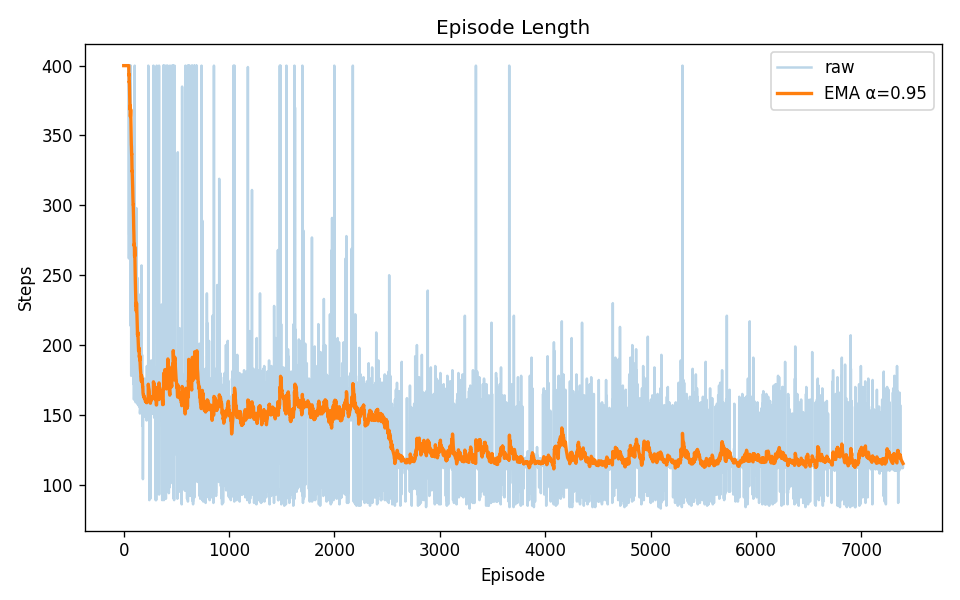
\includegraphics[width=0.7\linewidth]{figure/double_mountain_car/episode_length.png}
    \par
    \centering (a) 每轮步数
    \par
    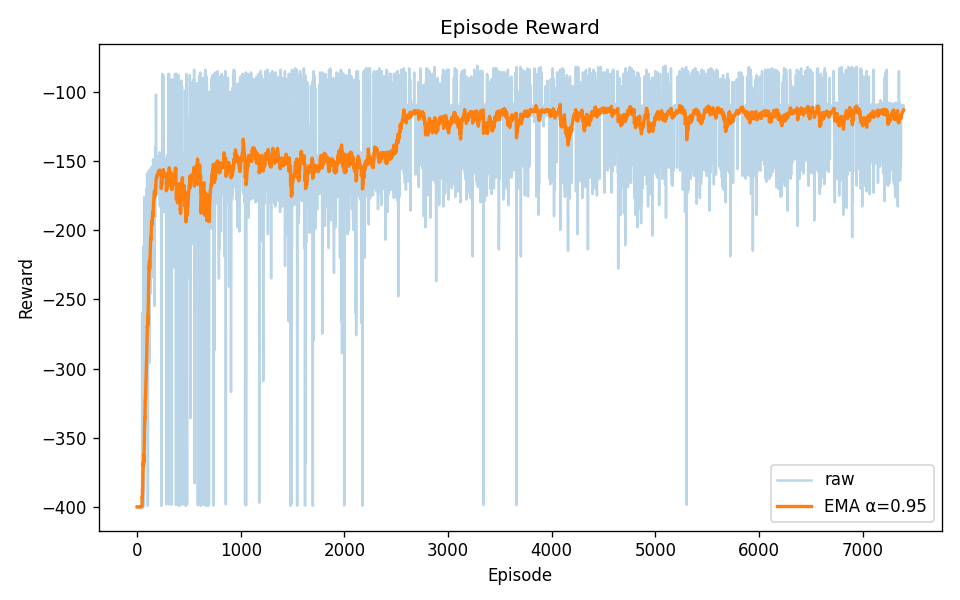
\includegraphics[width=0.7\linewidth]{figure/double_mountain_car/reward_curve.png}
    \par
    \centering (b) 收益曲线
    \par
    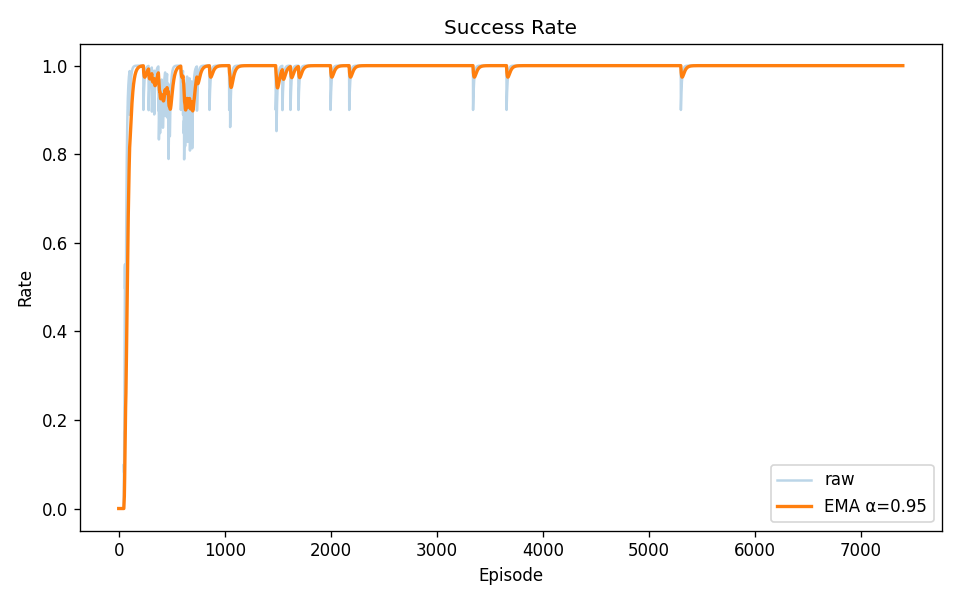
\includegraphics[width=0.7\linewidth]{figure/double_mountain_car/success_rate.png}
    \par
    \centering (c) 成功率
    \caption{Double Mountain Car 的训练结果曲线}
    \label{fig:ppo}
\end{figure}

本实验成功实现了基于 PPO 算法的 Double Mountain Car 问题训练,验证了 PPO 在多智能体离散动作空间中的学习能力。训练结果表明智能体能够有效协作,达成双车目标任务。

\subsection{参数设置}

本实验中的参数设置如表~\ref{tab:ppo-double-mountain-car-params} 所示:

\begin{table}[htbp]
\centering
\caption{PPO 算法在 Double Mountain Car 环境中的实验参数设置}
\label{tab:ppo-double-mountain-car-params}
\begin{tabular}{@{}lll@{}}
\toprule
\textbf{参数名称} & \textbf{含义} & \textbf{设置值} \\
\midrule
环境    & 训练使用的环境 & Double Mountain Car \\
状态空间维度    & 环境观测的特征数 & 4(两个小车的位置和速度) \\
动作空间维度    & 联合动作数量     & 9(两个小车各 3 个动作组合) \\
最大回合步数    & 每回合最大交互步数 & 400 \\
训练总步数  & PPO 训练总采样步数 & 1,000,000 \\
学习率  & 优化器初始学习率  & 0.0003 \\
折扣因子 \(\gamma\) & 奖励折扣系数      & 0.99 \\
批次大小    & PPO 每次更新批量大小 & 512 \\
时间步长 (n\_steps) & 每次 PPO 更新采样步数 & 1024 \\
剪切范围 (clip\_range)  & PPO 重要性采样裁剪范围 & 0.2 \\
奖励稠密化权重  & 位置变化奖励加权  & 2.0 \\
\bottomrule
\end{tabular}
\end{table}

\nocite{*}

\printbibliography[heading=bibintoc, title=\ebibname]
\appendix

\chapter{appendix}

\section{扫地机器人环境代码}\label{sec:sweeping-robot-env}

在这部分,展示我实现的扫地机器人的环境代码,代码接口符合 Gymnasium 的标准。

\begin{minted}[frame=single, fontsize=\small, linenos, breaklines]{python}
import gymnasium as gym
import numpy as np
import pygame
from gymnasium import spaces


class SweepingRobotEnv(gym.Env):
    metadata = {"render_modes": ["human", "rgb_array"], "render_fps": 15}

    def __init__(self, render_mode=None, size=5):
        super().__init__()
        self.size = size
        self.window_size = 512

        # 定义状态空间,在这里状态空间等同于观测空间
        self.observation_space = spaces.MultiDiscrete([size, size])
        
        spaces.Tuple(
            (spaces.Discrete(size), spaces.Discrete(size))
        )
        # 定义动作空间
        self.action_space = spaces.Discrete(4)

        # 记录机器人的位置,在后续的 reset 方法中会被初始化,并在 step 方法中更新
        # 此处仅仅是一个占位符,或者是冷启动状态
        self._agent_location = self.observation_space.sample()
        # 垃圾、充电桩和障碍物的位置
        self._trash_location = np.array([3, 4])
        self._charging_station_location = np.array([0, 0])
        self._obstacle_location = np.array([2, 2])

        assert render_mode is None or render_mode in self.metadata["render_modes"]
        self.render_mode = render_mode

        self.window = None
        self.clock = None

        self.icons = {}

        def load_icon(name, file):
            img = pygame.image.load(file)
            img = pygame.transform.scale(
                img,
                (int(self.window_size / self.size), int(self.window_size / self.size)),
            )
            self.icons[name] = img

        load_icon("robot", "icons/robot.png")
        load_icon("trash", "icons/trash.png")
        load_icon("charger", "icons/charger.png")
        load_icon("obstacle", "icons/block.png")

    def _get_obs(self):
        """返回当前 agent 的位置

        Returns:
            tuple: 当前 agent 的位置
        """
        return tuple(self._agent_location)

    def _get_info(self):
        """返回当前 agent 的位置与垃圾和充电桩的欧几里得距离信息

        Returns:
            list: 当前 agent 的位置与垃圾和充电桩的欧几里得距离信息
        """
        return {
            "distance_to_trash": np.sum(
                np.abs(self._agent_location - self._trash_location)
            ),
            "distance_to_charger": np.sum(
                np.abs(self._agent_location - self._charging_station_location)
            ),
        }

    def reset(self, init_pos=None, seed=None, options=None):
        # 处理 Gymnasium 内部的种子等
        super().reset(seed=seed)

        # 随机选择一个位置
        while True:
            initial_positions = self.observation_space.sample()
            if (
                not np.array_equal(initial_positions, self._charging_station_location)
                and not np.array_equal(initial_positions, self._trash_location)
                and not np.array_equal(initial_positions, self._obstacle_location)
            ):
                self._agent_location = initial_positions
                break

        observation = self._get_obs()
        info = self._get_info()

        # 对于 RecordVideo,不需要在 reset 时调用 _render_frame
        if self.render_mode == "human":
            self._render_frame()
        elif self.render_mode == "rgb_array":
            pass

        return observation, info

    def step(self, action):
        reward = 0.0  # 默认奖励,避免未赋值情况

        direction_vectors = {
            0: np.array([-1, 0]),  # 上
            1: np.array([1, 0]),  # 下
            2: np.array([0, -1]),  # 左
            3: np.array([0, 1]),  # 右
        }
        previous_location = np.copy(self._agent_location)
        self._agent_location = self._agent_location + direction_vectors[action]
        # 限定元素在 [0, size-1] 范围内
        self._agent_location = np.clip(self._agent_location, 0, self.size - 1)

        # 遇到墙不能走,用之前的位置代替
        if np.array_equal(self._agent_location, self._obstacle_location):
            self._agent_location = previous_location

        # 定义终止符号
        terminated = False
        if np.array_equal(self._agent_location, self._trash_location):
            reward = 5.0
            terminated = True
        elif np.array_equal(self._agent_location, self._charging_station_location):
            reward = 1.0
            terminated = True

        # 设置截断符号
        truncated = False
        observation = self._get_obs()
        info = self._get_info()

        # 对于 RecordVideo,不需要在 step 时主动调用 _render_frame
        # RecordVideo 包装器会在需要时调用 env.render()
        if self.render_mode == "human":
            self._render_frame()

        self._last_action = action
        self._last_reward = reward

        return observation, reward, terminated, truncated, info

    def render(self):
        # render 方法现在必须能处理 'rgb_array' 模式并返回图像
        if self.render_mode == "rgb_array":
            return self._render_frame()
        elif self.render_mode == "human":
            self._render_frame()  #  对于 human 模式,只渲染不返回
            return None  # Human mode render typically doesn't return
        else:
            super().render()  # 或者 gym.Env.render(self)

    def _render_frame(self):
        if self.window is None and self.render_mode == "human":
            pygame.init()
            pygame.display.init()
            self.window = pygame.display.set_mode(
                (self.window_size + 300, self.window_size)
            )
            pygame.display.set_caption("Sweeping Robot Env")

        if self.clock is None and self.render_mode == "human":
            self.clock = pygame.time.Clock()

        if pygame.display.get_init() == 0:
            pygame.init()

        for event in pygame.event.get():
            if event.type == pygame.QUIT:
                pygame.quit()
                self.close()

        # 初始化字体
        if not hasattr(self, "_info_font"):
            pygame.font.init()
            self._info_font = pygame.font.SysFont("Arial", 20)

        # 创建 canvas
        canvas = pygame.Surface((self.window_size + 300, self.window_size))
        canvas.fill((255, 255, 255))
        pix_square_size = self.window_size / self.size

        # 绘制元素图标
        def draw_icon(name, pos):
            if name in self.icons:
                icon = self.icons[name]
                canvas.blit(
                    icon,
                    (
                        pos[1] * pix_square_size,
                        (self.size - 1 - pos[0]) * pix_square_size,
                    ),
                )

        draw_icon("trash", self._trash_location)
        draw_icon("charger", self._charging_station_location)
        draw_icon("obstacle", self._obstacle_location)
        draw_icon("robot", self._agent_location)

        # 绘制网格
        for x in range(self.size + 1):
            pygame.draw.line(
                canvas,
                (128, 128, 128),
                (0, pix_square_size * x),
                (self.window_size, pix_square_size * x),
                width=1,
            )
            pygame.draw.line(
                canvas,
                (128, 128, 128),
                (pix_square_size * x, 0),
                (pix_square_size * x, self.window_size),
                width=1,
            )

        # 绘制右侧信息区域背景
        pygame.draw.rect(
            canvas,
            (240, 240, 240),
            pygame.Rect(self.window_size, 0, 300, self.window_size),
        )

        # 显示 agent 状态信息
        info_lines = []
        if hasattr(self, "_last_action"):
            action_name = ["UP", "DOWN", "LEFT", "RIGHT"][self._last_action]
            info_lines.append(f"Action: {action_name}")
        if hasattr(self, "_last_reward"):
            info_lines.append(f"Reward: {self._last_reward:.1f}")
        info_lines.append(
            f"Pos: ({int(self._agent_location[0] + 1)}, {int(self._agent_location[1] + 1)})"
        )

        for i, line in enumerate(info_lines):
            text_surf = self._info_font.render(line, True, (0, 0, 0))
            canvas.blit(text_surf, (self.window_size + 10, 20 + i * 30))

        # 渲染输出
        if self.render_mode == "human":
            self.window.blit(canvas, canvas.get_rect())
            pygame.event.pump()
            pygame.display.update()
            self.clock.tick(self.metadata["render_fps"])
            return None
        elif self.render_mode == "rgb_array":
            return np.transpose(
                np.array(pygame.surfarray.pixels3d(canvas)),
                axes=(1, 0, 2),
            )

    def close(self):
        if self.window is not None:
            pygame.display.quit()
            # pygame.quit() # pygame.quit() 会卸载所有 pygame 模块,如果其他地方还需要 pygame,可能会出问题
            self.window = None
        # 确保在所有 pygame 操作完成后才调用 pygame.quit()
        # 对于 RecordVideo, 只要 display 模块关闭即可,pygame.quit()可以在程序完全结束时调用
        if pygame.get_init():  # 检查 pygame 是否已初始化
            pygame.quit()


if __name__ == "__main__":
    pass

\end{minted}


\section{多开关匹配环境代码}\label{sec:multi-switch-env}

在这部分,展示我实现的多开关匹配的环境代码,代码接口符合 Gymnasium 的标准。

\begin{minted}[frame=single, fontsize=\small, linenos, breaklines]{python}
import sys
import time

import gymnasium as gym
import numpy as np
from gymnasium import spaces


class MultiSwitchEnv(gym.Env):
    metadata = {"render_modes": ["human"], "render_fps": 10}

    def __init__(self, render_mode=None, num_switches=3):
        super().__init__()
        self.num_switches = num_switches

        # 状态空间和动作空间都是 MultiBinary: 每个开关两个状态 0/1
        self.observation_space = spaces.MultiBinary(num_switches)
        self.action_space = spaces.MultiBinary(num_switches)  # 每个开关切或不切

        self.target_state = np.random.randint(0, 2, size=num_switches)
        self.state = None
        self.render_mode = render_mode
        self.steps = 0
        self.max_steps = 5

    def reset(self, seed=None, options=None):
        super().reset(seed=seed)
        self.state = self.np_random.integers(0, 2, size=self.num_switches)
        self.steps = 0
        return self.state.copy(), {}

    def step(self, action):
        self.steps += 1

        # 应用动作: 切换值(异或操作)
        self.state = (self.state + action) % 2

        done = np.array_equal(self.state, self.target_state)
        reward = 1.0 if done else -0.1
        truncated = self.steps >= self.max_steps

        return self.state.copy(), reward, done, truncated, {}

    def render(self):
        output = f"\rCurrent State: {self.state} | Target: {self.target_state}"
        sys.stdout.write(output)
        sys.stdout.flush()
        time.sleep(0.3)

    def close(self):
        pass
\end{minted}


\section{Double Mountain Car 环境代码}\label{sec:double-mountain-car-env}

在这部分,展示我实现的 Double Mountain Car,代码接口符合 Gymnasium 的标准。

\begin{minted}[frame=single, fontsize=\small, linenos, breaklines]{python}
import math
from typing import Optional

import gymnasium as gym
import numpy as np
from gymnasium import spaces
from gymnasium.envs.classic_control import utils


class DoubleMountainCarEnv(gym.Env):
    """
    Double Mountain Car Environment - Two cars that need to cooperate to reach the goal.

    ## Description
    This is an extension of the classic Mountain Car environment with two cars.
    Each car can be controlled independently, and they need to strategically
    accelerate to reach their respective goals.

    ## Observation Space
    The observation is a `ndarray` with shape `(4,)`:
    - [0]: position of car 1
    - [1]: velocity of car 1
    - [2]: position of car 2
    - [3]: velocity of car 2

    ## Action Space
    MultiDiscrete([3, 3]) - Each car has 3 actions:
    - 0: Accelerate to the left
    - 1: Don't accelerate
    - 2: Accelerate to the right
    """

    metadata = {
        "render_modes": [],
        "render_fps": 30,
    }

    def __init__(self, render_mode: Optional[str] = None, goal_velocity: float = 0):
        # Physical parameters
        self.min_position = -1.2
        self.max_position = 0.6
        self.max_speed = 0.07
        self.goal_position = 0.5
        self.goal_velocity = goal_velocity

        self.force = 0.001
        self.gravity = 0.0025

        # State bounds for both cars
        self.low = np.array(
            [
                self.min_position,
                -self.max_speed,  # Car 1
                self.min_position,
                -self.max_speed,  # Car 2
            ],
            dtype=np.float32,
        )

        self.high = np.array(
            [
                self.max_position,
                self.max_speed,  # Car 1
                self.max_position,
                self.max_speed,  # Car 2
            ],
            dtype=np.float32,
        )

        # Rendering
        self.render_mode = render_mode
        self.screen_width = 600
        self.screen_height = 400
        self.screen = None
        self.clock = None
        self.isopen = True

        # Action and observation spaces
        self.action_space = spaces.MultiDiscrete([3, 3])
        self.observation_space = spaces.Box(self.low, self.high, dtype=np.float32)

        # Initialize state
        self.state = None

    def step(self, action: np.ndarray):
        assert self.action_space.contains(action), (
            f"{action!r} ({type(action)}) invalid"
        )

        # Extract positions and velocities
        pos1, vel1, pos2, vel2 = self.state

        # Update car 1
        vel1 += (action[0] - 1) * self.force + math.cos(3 * pos1) * (-self.gravity)
        vel1 = np.clip(vel1, -self.max_speed, self.max_speed)
        pos1 += vel1
        pos1 = np.clip(pos1, self.min_position, self.max_position)
        if pos1 == self.min_position and vel1 < 0:
            vel1 = 0

        # Update car 2
        vel2 += (action[1] - 1) * self.force + math.cos(3 * pos2) * (-self.gravity)
        vel2 = np.clip(vel2, -self.max_speed, self.max_speed)
        pos2 += vel2
        pos2 = np.clip(pos2, self.min_position, self.max_position)
        if pos2 == self.min_position and vel2 < 0:
            vel2 = 0

        # Check termination - both cars need to reach the goal
        car1_at_goal = pos1 >= self.goal_position and vel1 >= self.goal_velocity
        car2_at_goal = pos2 >= self.goal_position and vel2 >= self.goal_velocity
        terminated = bool(car1_at_goal and car2_at_goal)

        # Reward: -1 per timestep, bonus when both reach goal
        reward = -1.0
        # Update state
        self.state = np.array([pos1, vel1, pos2, vel2], dtype=np.float32)

        if self.render_mode == "human":
            self.render()

        return self.state, reward, terminated, False, {}

    def reset(
        self,
        *,
        seed: Optional[int] = None,
        options: Optional[dict] = None,
    ):
        super().reset(seed=seed)

        # Initialize both cars at random positions
        low, high = utils.maybe_parse_reset_bounds(options, -0.6, -0.4)

        # Car 1 starts at a random position
        pos1 = self.np_random.uniform(low=low, high=high)
        vel1 = 0

        # Car 2 starts at a different random position
        pos2 = self.np_random.uniform(low=low, high=high)
        vel2 = 0

        self.state = np.array([pos1, vel1, pos2, vel2], dtype=np.float32)

        if self.render_mode == "human":
            self.render()

        return self.state, {}
\end{minted}


\section{针对扫地机器人环境的 SARAS 代码}\label{sec:saras}

我们对于扫地机器人问题,首先实现了 SARSA (State-Action-Reward-State-Action) 算法。
SARSA 是一种基于时间差分(Temporal Difference, TD)的强化学习算法,用于在智能体与环境交互过程中,学习一个状态-动作价值函数(\(Q\) 函数)。它是一个 \textbf{on-policy(依策略)} 的算法,意味着它学习的是当前行为策略下的 \(Q\) 值。

SARSA 的名字来自它更新公式中用到的五个元素:
\begin{itemize}
    \item \(S_t\):当前状态(State)
    \item \(A_t\):当前动作(Action)
    \item \(R_{t+1}\):执行动作后的即时奖励(Reward)
    \item \(S_{t+1}\):下一个状态(State)
    \item \(A_{t+1}\):在下一个状态选择的动作(Action)
\end{itemize}

SARSA 的基本更新公式为:
\[
    Q^{\texttt{new}} \left( s_t, a_t \right) \leftarrow  Q \left( s_t, a_t \right) + \alpha \left[ r_{t} + \gamma Q \left( s_{t+1}, a_{t+1} \right) - Q \left( s_t, a_t \right) \right]
\]
其中,\(\alpha\) 是学习率(learning rate),\(\gamma\) 是折扣因子(discount factor),衡量未来奖励的重要性。\(Q \left( S_t, A_t \right)\) 是状态-动作价值函数。
整个算法可以参考算法~\ref{ alg:sarsa}。

\begin{algorithm}[htbp]
\caption{SARSA 算法}\label{alg:sarsa}
\KwIn{学习率 \(\alpha\),折扣因子 \(\gamma\),探索率 \(\epsilon\),训练轮数 \(E\),最大步数 \(T\)}
\KwOut{动作-状态值函数 \(Q(s,a)\)}

初始化 \(Q\) 表为全零矩阵: \(Q(s,a) = \mathbf{0}_{\left|s\right|\times\left|a\right|}\)\;

\For{\( \text{episode} = 1 \) \KwTo \( E \)}{
    初始化环境状态 \( s_0 \)\;
    使用 \(\epsilon\)-greedy 策略,根据当前策略从状态 \(s_t\) 中选择动作 \(a_t\)例如 )\;
    \While{状态 \(s_t\) 不是终止状态 \textbf{or} t < T} {
        执行动作 \(a_t\),观察奖励 \(r_t\) 和下一个状态 \(s_{t+1}\)\;
        利用 \(\epsilon\)-greedy 策略 从状态 \(s_{t+1}\) 根据当前策略选择动作 \(a_{t+1}\)(例如 )\;
         生成随机数 \(p \sim \mathcal{U}(0,1)\)\;

        \eIf{\( p < \epsilon \)}{
            以等概率从动作集合 \( \mathcal{A} \) 中随机选择一个动作 \( a \)\;
        }{
            选择具有最大动作值的动作:\\
            \[ a \leftarrow \arg\max_{a \in \mathcal{A}} Q(s, a); \]
        }
        更新 \(Q\) 表 
        \[Q \left( s_t, a_t \right) \leftarrow  Q \left( s_t, a_t \right) + \alpha \left[ r_{t} + \gamma Q \left( s_{t+1}, a_{t+1} \right) - Q \left( s_t, a_t \right) \right];\]
        
        更新状态与动作
        \[s_t \leftarrow s_{t+1}, \qquad a_t \leftarrow a_{t+1};\]
    }
}
\Return{\( Q(s,a) \)}
\end{algorithm}

\subsection{算法实现细节}

具体实现代码参考附录~\ref{sec:saras}。
此处补充关键实现流程描述:
\begin{itemize}
    \item \textbf{状态映射}:使用 \textsf{state\_to\_index} 函数将二维坐标映射到 \(Q\) 表索引;
    \item \textbf{行为选择}:采取 \(\epsilon\)-greedy 策略在探索与利用之间平衡;
    \item \textbf{SARSA 更新}:在每一步中依据当前动作与下一个动作进行 \(Q\) 值更新;
    \item \textbf{训练结束条件}:达到最大步数或进入终止状态;
    \item \textbf{结果和策略可视化}:使用 matplotlib 绘制学习曲线,展示每轮的平均奖励。并将训练完成后将最终 \(Q\) 表策略渲染为箭头图示。
\end{itemize}

\subsection{实验结果与分析}

在这部分,展示使用 SARSA 方法控制扫地机器人的实验结果,包括策略可视化和学习曲线。

\subsubsection{策略可视化}

通过 \textsf{visualize\_policy\_from\_q} 函数生成的策略图如下所示(见图~\ref{fig:sarsa_policy})。其中箭头方向表示在各状态下的最优动作,我们可以清楚的从策略图中看到智能体能够顺利收集垃圾,获得最好的收益 \(5\),而不是在某些格子处陷入局部最优(获得充电站的收益 \(1\))。

\begin{figure}[htbp] 
    \centering 
    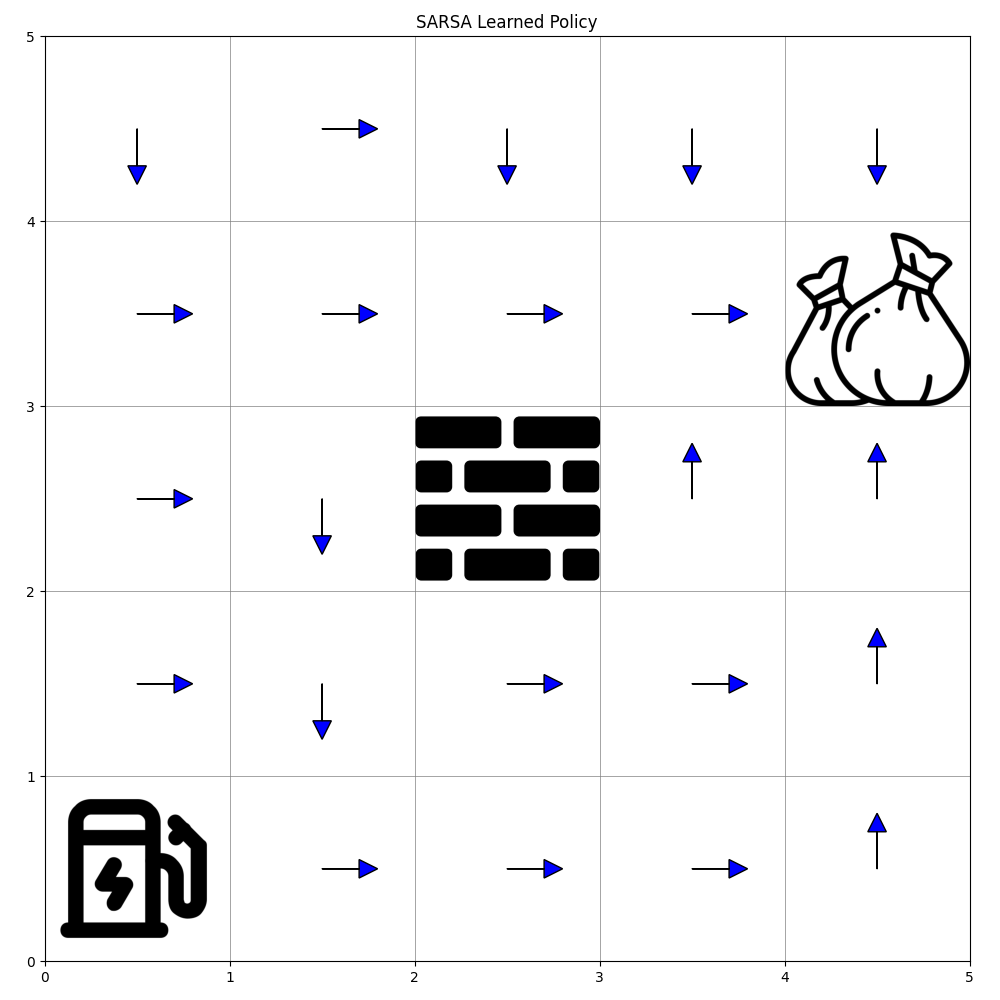
\includegraphics[width=0.5\textwidth]{figure/sweep_robot/sarsa/policy_visualization.png} 
    \caption{SARSA 策略可视化图}\label{fig:sarsa_policy} 
\end{figure}

\subsubsection{学习曲线}

训练过程中的奖励、步数与成功率变化如下图~\ref{fig:sarsa_training} 所示:
其中,我们展示了收益、步数和成功率的变化趋势。
其中我们定义成功率(Success Rate)为机器人成功达到垃圾位置而不是充电站的次数占所有试验次数的比例。
并使用了参数为 \(0.99\) 的指数移动平均值(EMA)进行展示。
可以看到,随着训练的进行,智能体的平均奖励逐渐上升,步数逐渐减少,成功率也在不断提高。这表明智能体逐渐学会了如何在环境中有效地收集垃圾而不是直接去充电站。
初期智能体尝试较多,步数波动较大;后期逐渐收敛。
我们发现成功率呈上升趋势,训练后期趋于稳定,表明智能体学会有效完成任务(捡拾垃圾而不是直接去充电站)。
一开始位置的 \(100\) \% 成功率和总步数为 \(0\) 是因为随机性导致智能体容易直接在垃圾位置附近开始,捡拾成功。

\begin{figure}[htbp] 
    \centering 
    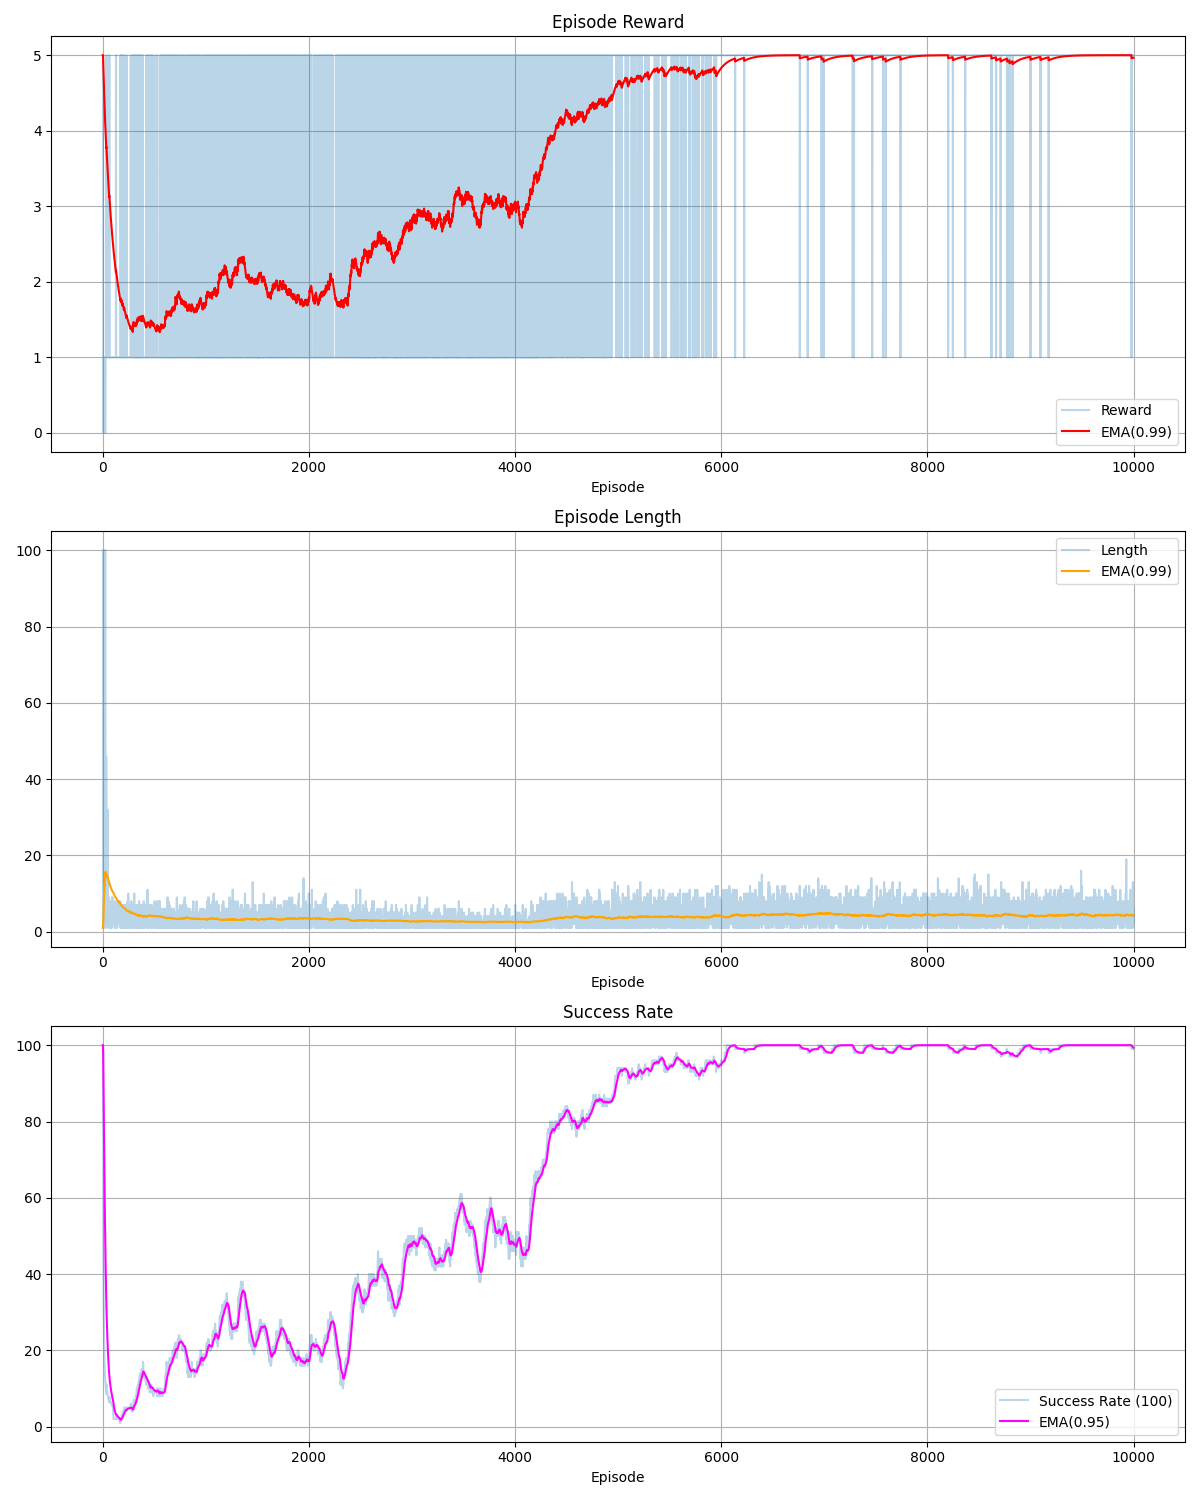
\includegraphics[width=0.8\textwidth]{figure/sweep_robot/sarsa/training_results.png} 
    \caption{SARSA 训练过程统计曲线}\label{fig:sarsa_training} 
\end{figure}

\subsection{参数设置}

本实验中的参数设置如下:
\begin{table}[htbp]
\centering
\caption{SARSA算法主要参数设置}
\label{tab:sarsa_three_line}
\begin{tabular}{ccc}
\toprule
\textbf{参数} & \textbf{取值} & \textbf{说明} \\
\midrule
\(\alpha\)(学习率) & \(0.1\) & 控制每步 \(Q\) 值更新的幅度,决定新经验对旧知识的替代程度。 \\
\(\gamma\)(折扣因子) & \(0.99\) & 衡量未来奖励对当前决策的重要性,越接近 \(1\) 表示越注重长期收益。 \\
\(\epsilon\)(探索率) & \(0.1\) & \(\epsilon\)-贪婪策略中用于随机探索的概率,平衡探索与利用。 \\
总回合数(Episodes) & \(10000\) & 智能体与环境交互的总轮数,较大值有助于收敛策略。 \\
最大步长(per episode) & \(100\) & 每回合允许的最大步数,防止陷入死循环。 \\
\bottomrule
\end{tabular}
\end{table}

\section{针对扫地机器人环境的 REINFORCE 策略梯度算法代码}\label{sec:REINFORCE}

该实验部分采用 REINFORCE 策略梯度算法~\cite{DBLP:journals/ml/Williams92} 对清扫机器人任务进行训练。

REINFORCE 算法是一种基于策略梯度的强化学习算法,用于求解策略优化问题。
它属于无模型强化学习算法,直接通过策略来选择动作并进行优化,而不是通过值函数或环境模型来估计动作的回报。
在传统的值函数方法(如 \(Q\)-Learning 或 SARSA)中,核心目标是学习一个状态-动作值函数 \(Q \left( s, a \right)\),再通过贪婪策略派生出最优行为。

但一般认为在复杂任务中,值函数方法往往不易收敛,且对连续动作空间支持不佳。为此,引入了 \textbf{策略梯度方法(Policy Gradient Methods)},直接建模并优化一个参数化策略 \(\pi_{\theta} \left( a \mid s \right) \),以提高学习的稳定性与泛化能力。
在这一基础上,Williams et al. 提出了 REINFORCE,这也是最早的、也是最简单的一种蒙特卡洛策略梯度算法。其核心思想是:
\begin{itemize}
    \item “利用完整轨迹中的实际奖励来指导策略的改进,增强出现好结果的动作概率,抑制差结果的动作。”
\end{itemize}

策略梯度的优化目标为最大化期望总回报:
\begin{equation}\label{eq:policy_gradient_objective}
    \mathbf{J} \left( \theta \right) = \mathbb{E}_{\tau \sim \pi_{\theta}} \left[ R \left( \tau \right) \right]
\end{equation}
其中,\(\tau = \left(s_0, a_0, r_1, \dots, s_T, a_T, r_{T+1}\right)\) 表示一个完整轨迹,\(R \left( \tau \right)\) 为轨迹总回报。
通过对数概率技巧(log-derivative trick),策略梯度可以表示为:
\begin{equation}\label{eq:policy_gradient-log}
    \nabla_{\theta} \mathbf{J} \left( \theta \right) = \mathbb{E}_{\tau \sim \pi_{\theta}} \left[ \sum_{\pi_\theta} \nabla_{\theta} \log \pi_{\theta} \left( a_t \mid s_t \right) \cdot R_t \right]
\end{equation}
其中 \(R_t\) 是从时刻 \(t\) 开始的累计折扣奖励:
\[
    R_t = \sum_{k=0}^{T-t} \gamma^k r_{t+k+1}
\]
这种形式意味着——在每一步中,提高当时策略选择该动作的概率,按当前回报加权。

REINFORCE 的梯度估计是无偏的,但由于直接用回报 \(R\) 乘以 \(\log\) 概率,导致方差较大,训练不稳定。
为此,常引入 baseline(基线) 来降低方差,所以公式 (\ref{eq:policy_gradient_objective}) 可以改写为:
\begin{equation}\label{eq:policy_gradient_objective-log_baseline}
    \mathbf{J} \left( \theta \right) = \nabla_{\theta} \mathbf{J} \left( \theta \right) = \mathbb{E}_{\tau \sim \pi_{\theta}} \left[ \sum_{\pi_\theta} \nabla_{\theta} \log \pi_{\theta} \left( a_t \mid s_t \right) \cdot \left( R_t - b_t \right) \right]
\end{equation}
在本文中,我们的实现就是如公式 (\ref{eq:policy_gradient_objective-log_baseline}) 加入了 baseline 的 REINFORCE 算法。
算法归纳参考算法~\ref{agl:REINFORCE_replay},其中包含熵正则项(Entropy Regularization)来鼓励策略的探索性,算法中参数的含义和具体实现参考后文中的小节~\ref{subsubsec:REINFORCE-state-action} 部分。

\begin{algorithm}[htbp]
\caption{带经验回放的 REINFORCE 策略梯度算法}\label{agl:REINFORCE_replay}
\KwIn{策略网络 \( \pi_\theta(a \mid s) \),折扣因子 \( \gamma \),回放权重 \( \beta \),初始熵系数 \( \lambda_{\texttt{init}} \),最小熵系数 \( \lambda_{\texttt{min}} \),学习率 \( \alpha \),最大训练轮数 \( E \),经验缓存上限 \( N \),重放池大小 \(M\),最大步数 \( T \),经验回放频率 \( K \)}
\KwOut{最优策略参数 \( \theta \)}

初始化成功轨迹缓存池:\( \mathcal{M} \leftarrow \emptyset \)\;

\For{\( \text{episode} = 1 \) \KwTo \( E \)}{
    初始化环境状态 \( s_0 \)\;
    初始化轨迹存储列表:\( S \leftarrow [] \),\( A \leftarrow [] \),\( R \leftarrow [] \)\;

    \While{未终止}{
        采样动作:\( a_t \sim \pi_\theta(\cdot \mid s_t) \)\;
        执行动作,获得奖励 \( r_t \) 和新状态 \( s_{t+1} \)\;
        记录:\( S \gets S \cup \{s_t\} \),\( A \gets A \cup \{a_t\} \),\( R \gets R \cup \{r_t\} \)\;
    }

    \If{\( 成功拾取垃圾 \)}{
        将 \( (S, A, R) \) 存入成功缓存 \( \mathcal{M} \)\;
        若 \( |\mathcal{M}| > N \),则移除最旧轨迹\;
    }

    \For{\( t = 0 \) \KwTo \( T \)}{
        计算折扣回报:
        \[
        R_t \leftarrow \sum_{k=0}^{T - t} \gamma^k r_{t + k} ;
        \]
    }

    计算当前轨迹损失:
    \For{\( t = 0 \) \KwTo \( T \)}{
        \[
        \mathcal{L}_t \left( \theta \right) = -  \sum_{t=0}^{T} \left[ \hat{A}_t \log \pi_{\theta} \left( a_t \mid s_t \right) + \lambda \cdot \mathcal{H} \left( \pi_{\theta} \left( a_t \mid s_t \right) \right) \right], \quad \lambda = \max \left( \lambda_{\texttt{min}}, \lambda_{\texttt{init}} \cdot \left( 1 - \frac{e}{E} \right) \right)
        \]
    }

    \If{\( \text{episode} \bmod K = 0 \) \textbf{and} \( |\mathcal{M}| > 0 \)}{
        从 \( \mathcal{M} \) 中抽取一条成功轨迹 \( (S^{\prime}, A^{\prime}, R^{\prime}) \)\;
        重复上面步骤,计算其对应的回报 \( R^{\prime}_t \) 和损失 \( \mathcal{L}^{\prime}_t \)\;
        合并总损失:\[ \mathcal{L}_t \leftarrow \mathcal{L}_t + \beta \cdot \sum_t \mathcal{L}^{\prime}_t; \]
        \For{\( t = 0 \) \KwTo \( M \)}{
            \textbf{累加:} \( \mathcal{L}_t \leftarrow \mathcal{L}_t + \beta \cdot \mathcal{L}_t^{\prime} \)
        }
    }

    更新策略参数:
    \[
    \theta \leftarrow \theta - \alpha \nabla_\theta \sum_{t=0}^T \mathcal{L}_t
    \]
}
\Return{\( \theta \)}
\end{algorithm}


\subsection{算法实现细节}

在这一节中,我们具体展示我们代码实现的细节。具体实现代码参考附录~\ref{sec:REINFORCE}。

\subsubsection{策略网络结构设计}

策略 \(\pi_\theta \left( a \mid s\right)\) 通常用神经网络建模,输出为一个概率分布(softmax),从中采样动作。
对于此处,本实验使用一个三层全连接神经网络(\textsf{PolicyNetwork} 类)作为策略函数,输入为 one-hot 编码后的状态向量,输出为动作概率分布。网络结构如下:
\begin{itemize}
    \item 输入层:状态维度(\(5 \times 5\)网格,\(25\) 维)
    \item 两个隐藏层:各 \(64\) 个神经元
    \item 输出层:\(4\) 个动作方向(上、下、左、右)的 \texttt{Softmax} 概率
    \item 网络权重使用 Xavier 初始化,激活函数采用 ReLU,以确保训练稳定性。
\end{itemize}
具体函数如下:
\begin{minted}[fontsize=\small, breaklines]{python}
class PolicyNetwork(nn.Module):
    def __init__(self, input_size, hidden_size, output_size):
        super(PolicyNetwork, self).__init__()
        self.fc1 = nn.Linear(input_size, hidden_size)
        self.fc2 = nn.Linear(hidden_size, hidden_size)
        self.fc3 = nn.Linear(hidden_size, output_size)

        # 初始化权重
        nn.init.xavier_uniform_(self.fc1.weight)
        nn.init.xavier_uniform_(self.fc2.weight)
        nn.init.xavier_uniform_(self.fc3.weight)

        nn.init.zeros_(self.fc1.bias)
        nn.init.zeros_(self.fc2.bias)
        nn.init.zeros_(self.fc3.bias)

    def forward(self, x):
        x = F.relu(self.fc1(x))
        x = F.relu(self.fc2(x))
        x = self.fc3(x)
        # 添加数值稳定性
        # x = torch.clamp(x, min=-10, max=10)  # 防止过大的 logits
        return F.softmax(x, dim=-1)
\end{minted}

\subsubsection{状态表示与动作采样}\label{subsubsec:REINFORCE-state-action}

状态通过 \textsf{state\_to\_tensor()} 函数转换为 one-hot 编码张量,输入策略网络后返回 \texttt{Softmax} 输出作为动作概率。
通过 \textsf{torch.distributions.Categorical} 分布进行动作采样,以保持策略的随机性和探索能力。

\begin{minted}[fontsize=\small, breaklines]{python}
...
def state_to_tensor(state, size):
    """将状态转换为 one-hot 编码的张量"""
    row, col = state
    state_vector = torch.zeros(size * size)
    state_vector[row * size + col] = 1
    return state_vector
...
# 采样动作
m = Categorical(action_probs)
...
\end{minted}

\subsection{回报计算与损失函数设计}

使用 \textsf{compute\_returns()} 函数计算每一步的折扣回报:
\[
    R_t = \sum_{k=0}^{T-t} \gamma^k r_{t+k+1}
\]

为减小训练不稳定性,引入 baseline(平均回报)并标准化优势函数:

\[
    A_t = R_t - \bar{R}, \qquad \hat{A}_t = \frac{A_t - \mathbb{E}[A_t]}{\sqrt{\text{Var}(A_t)} + \varepsilon}
\]
其中 \(\mathbb{E}[A_t]\) 是优势函数 \(A\) 的均值,\(\text{Var}(A_t)\) 是方差,\(\varepsilon\) 是一个小常数(如 \(1e-8\))以避免除零错误。
并且我们引入了熵正则项(Entropy Regularization):在策略梯度方法(尤其是 REINFORCE)中,智能体在训练早期往往面临策略收敛过快、陷入局部最优的问题。为缓解这一现象,常引入熵正则项(Entropy Regularization)来鼓励策略的随机性和探索性。
熵是衡量概率分布不确定性的度量。在策略网络中,若某一时刻的动作概率分布越平均,其熵越高,说明策略具有更强的探索能力;反之,若某一动作概率接近 \(1\),则熵趋于 \(0\),表示策略已趋于确定性,可能导致提前陷入“贪婪”。
对于策略 \( \pi_{\theta} \left( a \mid s \right) \) 的动作分布,其熵定义为:
\begin{equation}
    \mathcal{H} \left( \pi_{\theta} \left( a \mid s \right) \right) = - \sum_a \pi_{\theta} \left( a \mid s \right) \log \pi_{\theta} \left( a \mid s \right)
\end{equation}
熵越大,说明动作分布越均匀,策略越具有“探索性”。
在策略优化中,我们将熵项作为额外奖励项添加至原始损失函数中,从而形成如下形式的目标函数,得到最终损失为:
\begin{equation}
    \mathcal{L} \left( \theta \right) = - \mathbb{E}_{\tau \sim \pi_{\theta}} \left[ \sum_{t=0}^{T} \hat{A}_t \log \pi_{\theta} \left( a_t \mid s_t \right) + \lambda \cdot \mathcal{H} \left( \pi_{\theta} \left( a_t \mid s_t \right) \right) \right]
\end{equation}
其中 \(\lambda\) 为熵正则项的权重系数,并会动态调整:
\[
    \lambda = \max \left( \lambda_{\texttt{min}}, \lambda_{\texttt{init}} \cdot \left( 1 - \frac{e}{E} \right) \right)
\]
其中,\(e\) 为当前训练的 episode 编号;\(E\) 为总训练轮数(即 episodes);\(\lambda_{\texttt{min}}\) 为初始熵系数(代码中为 \(0.8\));\(\lambda_{\texttt{init}}\) 为最小熵系数(代码中为 \(0.1\));早期训练阶段 \(\frac{e}{E} \approx 0 \Rightarrow \lambda \approx 0.8\),鼓励探索。训练中期至后期 \(\frac{e}{E} \approx 1 \Rightarrow \lambda \to 0.1\),逐步转向稳定策略。

代码中,熵正则项的实现如下:
\begin{minted}[fontsize=\small, breaklines]{python}
...
entropy_coef = max(0.1, 0.8 * (1 - episode / episodes))
...
entropy_bonus += m.entropy() * entropy_coef
...
loss = torch.stack(policy_loss).sum() - entropy_bonus
...
\end{minted}

\subsection{学习率调度与稳定机制}

\subsubsection{学习率调度}

实验中,优化器采用 \texttt{Adam},初始学习率为 \(0.001\),并通过 StepLR 每 \(1000\) 轮衰减至 \(95\)\%。
同时为防止梯度爆炸,引入梯度裁剪(最大范数为 \(5.0\))。此外,在每 \(50\) 轮训练中使用一次经验回放,利用之前成功轨迹进一步强化学习。

\subsubsection{经验回放机制}

在训练过程中,智能体通过与环境交互收集状态、动作、奖励等信息,并将这些信息存储在经验回放缓冲区中。
依赖于这些存储信息,我实现了\textbf{“成功经验回收机制”} 以完善训练:只保存过去成功到达目标(即成功回收垃圾)的完整轨迹,保留最近 \(10\) 条;每 \(50\) 轮训练时,从这些轨迹中随机挑选一条,加入当前训练 loss 中一同反向传播。

\rcomment[什么是“经验回收机制”?]{在强化学习中,\textbf{经验回放(Experience Replay)}指的是将过去的一些经验(即状态、动作、奖励等轨迹)保存下来,在后续训练中反复使用,而不是每次都只依赖当前的样本。}

保存成功轨迹部分代码如下:

\begin{minted}[fontsize=\small, breaklines]{python}
if total_reward >= 5:
    success_count += 1
    recent_successes.append({
        "states": states.copy(),
        "actions": actions.copy(),
        "rewards": rewards.copy()
    })
    if len(recent_successes) > 10:
        recent_successes.pop(0)
\end{minted}

每隔 \(50\) 轮回放一次

\begin{minted}[fontsize=\small, breaklines]{python}
if len(recent_successes) > 0 and episode % 50 == 0:
    success_traj = recent_successes[np.random.randint(len(recent_successes))]
    ...
    for state, action, advantage in zip(...):
        ...
        policy_loss.append(-m.log_prob(action) * advantage * 0.5)
\end{minted}

\subsection{参数设置}

本实验的参数设置可参考表~\ref{tab:reinforce-params}。

\begin{table}[htbp]
\centering
\caption{REINFORCE算法实验参数设置}
\label{tab:reinforce-params}
\begin{tabular}{@{}lll@{}}
\toprule
\textbf{参数名称} & \textbf{含义} & \textbf{设置值} \\
\midrule
Grid Size & 环境网格大小 & \( 5 \times 5 \) \\
Input Size & 状态维度(One-hot 编码) & \( 25 \) \\
Hidden Size & 隐藏层神经元数 & \( 64 \) \\
Output Size & 动作空间维度(上下左右) & \( 4 \) \\
Learning Rate & 学习率 & \( 0.001 \) \\
Optimizer & 优化器类型 & Adam \\
Discount Factor \(\gamma\) & 折扣因子 & \( 0.995 \) \\
Entropy Coefficient \(\lambda\) & 熵正则化系数 & \( 0.8 \rightarrow 0.1 \)(线性递减) \\
Gradient Clipping & 梯度裁剪最大范数 & \( 5.0 \) \\
Scheduler & 学习率调度器 & StepLR,每 \( 1000 \) 轮乘 \( 0.95 \) \\
Episodes & 总训练轮数 & \( 10000 \) \\
Max Steps / Episode & 每回合最大步数 & 动态增长,\( 50 \rightarrow 100 \) \\
EMA Smoothing Factor & EMA 平滑系数(奖励/步数) & \( 0.95 \sim 0.99 \) \\
Replay Frequency & 成功轨迹经验回放频率 & 每 \( 50 \) 轮一次 \\
Replay Buffer Size & 成功轨迹最大存储数量 & \( 10 \) 条 \\
Replay Weight & 成功轨迹回放权重 & \( 0.5 \) \\
\bottomrule
\end{tabular}
\end{table}

\subsubsection{实验结果与分析}

\subsubsection{策略可视化}

通过 \textsf{visualize\_policy} 函数生成的策略图如下所示(见图~\ref{fig:REINFORCE_policy})。其中箭头方向表示在各位置动作策略(只绘制概率 \(> 0.1\) 的策略。

\begin{figure}[htbp] 
    \centering 
    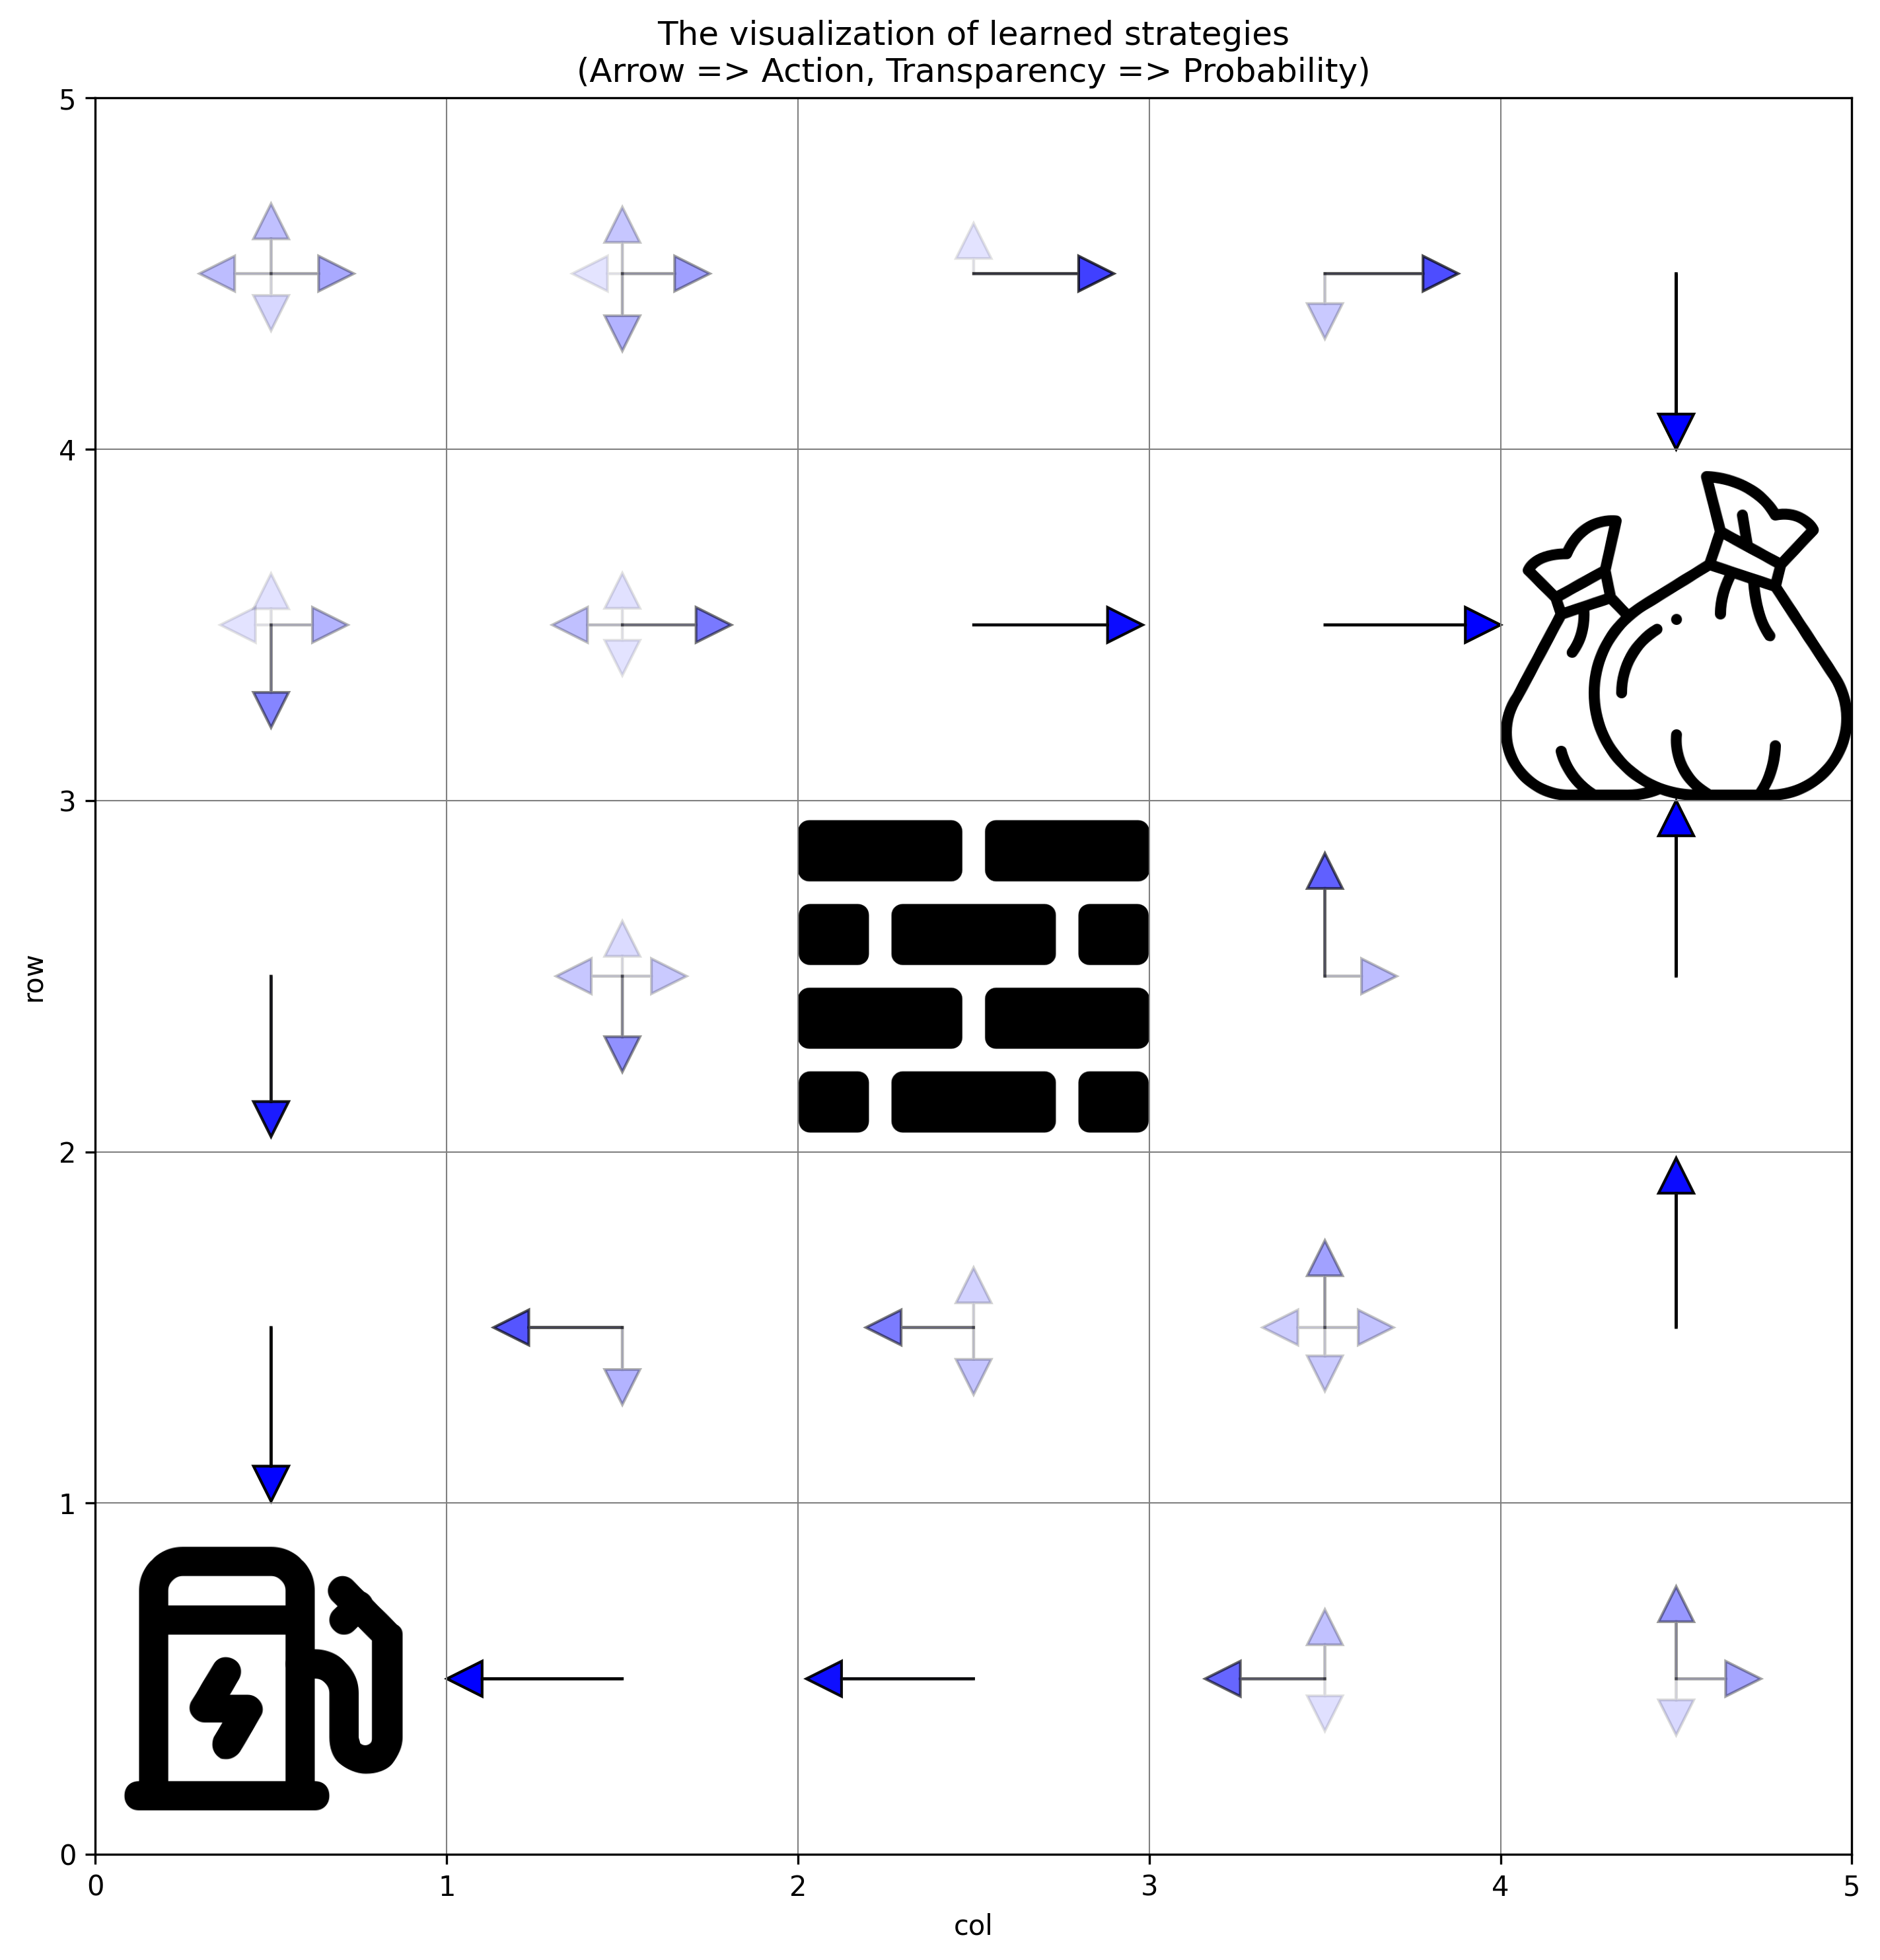
\includegraphics[width=0.5\textwidth]{figure/sweep_robot/REINFORCE/policy_visualization.png} 
    \caption{REINFORCE 策略梯度算法的策略可视化图}\label{fig:REINFORCE_policy} 
\end{figure}

\subsubsection{学习曲线}

本实验的学习曲线如图~\ref{fig:REINFORCE_training} 所示。我们展示了收益、步数和成功率的变化趋势。

\begin{figure}[htbp] 
    \centering 
    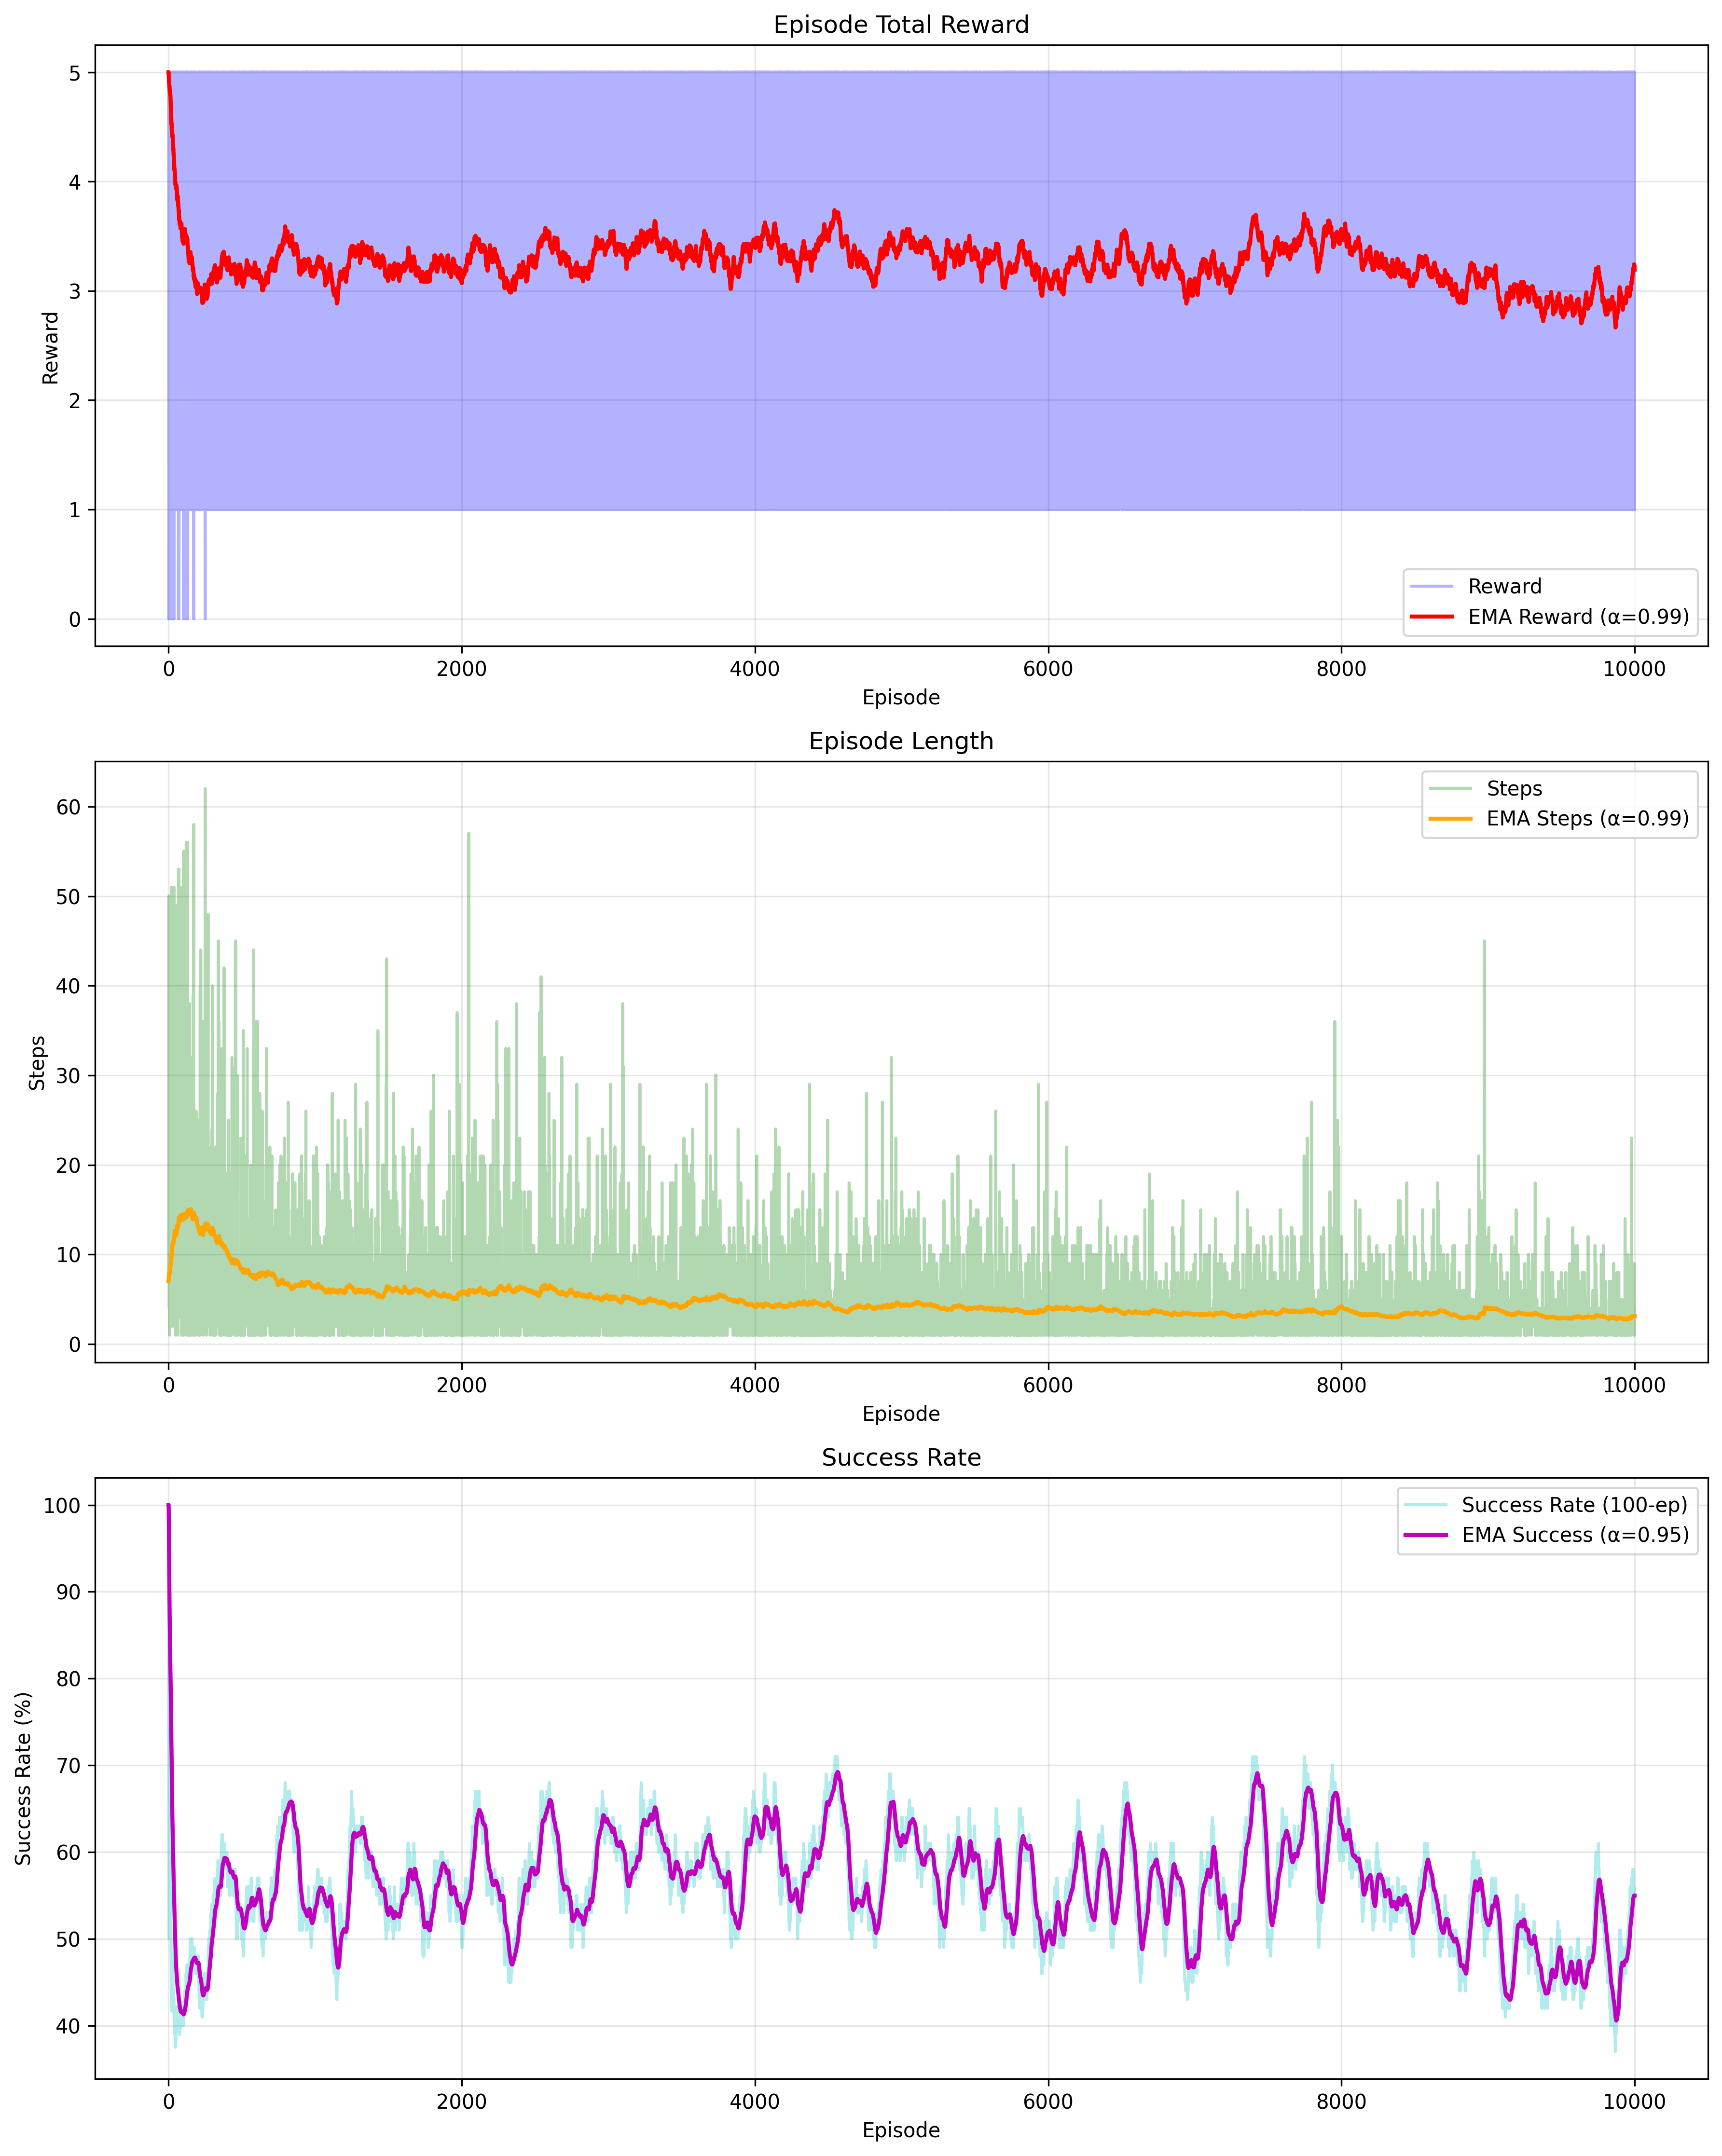
\includegraphics[width=0.8\textwidth]{figure/sweep_robot/REINFORCE/training_results.png} 
    \caption{REINFORCE 策略梯度算法的策略可视化图}\label{fig:REINFORCE_training} 
\end{figure}

可以发现,REINFORCE 算法在训练过程中,平均奖励水平较低,且波动较大。智能体在充电站附近停留时间过长,导致平均奖励水平未能有效提升,对于 SARAS 算法的表现较差。

\subsubsection{总结}

分析表明,REINFORCE 策略梯度算法在当前环境下未能习得有效的策略。
尽管智能体在训练过程中能够逐步收集垃圾,但其在充电站停留时间过长,导致平均奖励水平较低。
如图~\ref{fig:REINFORCE_policy} 所示,机器人越接近充电站,其选择充电而非收集垃圾的倾向越明显,这表明智能体可能在学习过程中陷入了局部最优解。

究其原因,核心问题在于环境奖励的稀疏性:仅在充电桩和垃圾位置提供奖励,使得智能体难以学习最优策略。其决策严重依赖轨迹末端状态,一旦习得“快速终止回合”的行为模式,便容易形成次优策略。

此外,REINFORCE 算法固有的特性也加剧了这一问题:
\begin{itemize}
    \item 回合制更新限制:算法需等待整个回合结束后才能获得总回报。在奖励稀疏或环境复杂的情况下,这显著增加了陷入次优策略的风险。
    \item  \textbf{反馈延迟}:由于回报基于回合总奖励,中间决策的优劣无法即时反馈给智能体。智能体需待回合结束方能评估决策正确性。若关键决策发生于回合后期,将导致梯度更新延迟,阻碍策略及时修正。
    \item \textbf{稀疏奖励}:在仅终点(垃圾/充电桩)提供奖励的稀疏环境下,智能体需经历较长路径才能获得有效信息,极易因探索不足而固守次优策略。
    \item \textbf{更新噪声与不稳定性}:依赖整条轨迹回报进行全局更新,使得梯度易受随机噪声干扰,导致训练过程波动较大,难以收敛至全局最优策略。
\end{itemize}

REINFORCE 算法在这种环境下的收敛速度较慢,且容易受到高方差的影响,导致学习不稳定。

\section{针对多开关匹配环境的 \(Q\)-learning 算法代码}\label{sec:q-learning}

在这部分,展示我实现的对于多开关匹配环境的智能体 \(Q\)-learning 实现代码。

\begin{minted}[frame=single, fontsize=\small, linenos, breaklines]{python}
import os
from collections import deque

import matplotlib.pyplot as plt
import numpy as np

from multi_switch_env import MultiSwitchEnv


class TrainingMonitor:
    """训练监控器,记录各种指标用于绘图"""

    def __init__(self):
        self.episode_rewards = []
        self.episode_lengths = []
        self.q_value_mean = []
        self.q_value_max = []
        self.success_rate = deque(maxlen=20)  # 滑动窗口记录最近 20 个 episode 的成功率
        self.epsilon_values = []

    def record_episode(self, total_reward, episode_length, success):
        self.episode_rewards.append(total_reward)
        self.episode_lengths.append(episode_length)
        self.success_rate.append(1.0 if success else 0.0)

    def record_q_values(self, q_table):
        self.q_value_mean.append(np.mean(q_table))
        self.q_value_max.append(np.max(q_table))

    def record_epsilon(self, epsilon):
        self.epsilon_values.append(epsilon)

    def compute_ema(self, data, alpha=0.9):
        """计算指数加权移动平均(EMA)"""
        ema = np.zeros_like(data, dtype=float)
        if len(data) > 0:
            ema[0] = data[0]
            for i in range(1, len(data)):
                ema[i] = alpha * ema[i - 1] + (1 - alpha) * data[i]
        return ema

    def plot_results(self, save_path="/multi_switch/training_results.png"):
        """绘制训练结果的综合图表"""
        fig, axes = plt.subplots(2, 3, figsize=(15, 10))
        fig.suptitle("Multi-Switch Environment Training Metrics", fontsize=16)

        # 设置统一的EMA参数
        ema_alpha = 0.95

        # 1. Episode Rewards
        ax1 = axes[0, 0]
        ax1.plot(
            self.episode_rewards,
            alpha=0.3,
            color="blue",
            linewidth=1,
            label="Raw Rewards",
        )
        # 添加EMA平滑线
        if len(self.episode_rewards) > 1:
            ema_rewards = self.compute_ema(self.episode_rewards, ema_alpha)
            ax1.plot(ema_rewards, "b-", linewidth=2.5, label=f"EMA ($\alpha$={ema_alpha})")
        ax1.set_xlabel("Episode")
        ax1.set_ylabel("Total Reward")
        ax1.set_title("Episode Rewards Over Time")
        ax1.legend()
        ax1.grid(True, alpha=0.3)

        # 2. Episode Lengths
        ax2 = axes[0, 1]
        ax2.plot(self.episode_lengths, "g-", alpha=0.3, linewidth=1, label="Raw Steps")
        if len(self.episode_lengths) > 1:
            ema_lengths = self.compute_ema(self.episode_lengths, ema_alpha)
            ax2.plot(ema_lengths, "g-", linewidth=2.5, label=f"EMA ($\alpha$={ema_alpha})")
        ax2.set_xlabel("Episode")
        ax2.set_ylabel("Steps")
        ax2.set_title("Episode Length (Steps to Complete)")
        ax2.legend()
        ax2.grid(True, alpha=0.3)

        # 3. Success Rate
        ax3 = axes[0, 2]
        if len(self.success_rate) > 0:
            success_rates = []
            for i in range(len(self.episode_rewards)):
                end_idx = min(i + 1, len(self.success_rate))
                start_idx = max(0, end_idx - 20)
                if end_idx > start_idx:
                    rate = sum(list(self.success_rate)[start_idx:end_idx]) / (
                        end_idx - start_idx
                    )
                    success_rates.append(rate * 100)
            ax3.plot(
                success_rates, "c-", alpha=0.3, linewidth=1, label="20-Episode Window"
            )
            if len(success_rates) > 1:
                ema_success = self.compute_ema(success_rates, ema_alpha)
                ax3.plot(ema_success, "b-", linewidth=2.5, label=f"EMA ($\alpha$={ema_alpha})")
        ax3.set_xlabel("Episode")
        ax3.set_ylabel("Success Rate (%)")
        ax3.set_title("Success Rate")
        ax3.legend()
        ax3.grid(True, alpha=0.3)
        ax3.set_ylim([0, 105])

        # 4. Q-Value Mean
        ax4 = axes[1, 0]
        ax4.plot(self.q_value_mean, "purple", alpha=0.3, linewidth=1, label="Raw Mean")
        if len(self.q_value_mean) > 1:
            ema_q_mean = self.compute_ema(self.q_value_mean, ema_alpha)
            ax4.plot(
                ema_q_mean, color="purple", linewidth=2.5, label=f"EMA ($\alpha$={ema_alpha})"
            )
        ax4.set_xlabel("Episode")
        ax4.set_ylabel("Mean Q-Value")
        ax4.set_title("Average Q-Value Over Time")
        ax4.legend()
        ax4.grid(True, alpha=0.3)

        # 5. Q-Value Max
        ax5 = axes[1, 1]
        ax5.plot(self.q_value_max, "orange", alpha=0.3, linewidth=1, label="Raw Max")
        if len(self.q_value_max) > 1:
            ema_q_max = self.compute_ema(self.q_value_max, ema_alpha)
            ax5.plot(
                ema_q_max, color="orange", linewidth=2.5, label=f"EMA ($\alpha$={ema_alpha})"
            )
        ax5.set_xlabel("Episode")
        ax5.set_ylabel("Max Q-Value")
        ax5.set_title("Maximum Q-Value Over Time")
        ax5.legend()
        ax5.grid(True, alpha=0.3)

        # 6. Epsilon Decay
        ax6 = axes[1, 2]
        if self.epsilon_values:
            ax6.plot(
                self.epsilon_values, "red", alpha=0.3, linewidth=1, label="Raw Epsilon"
            )
            if len(self.epsilon_values) > 1:
                ema_epsilon = self.compute_ema(self.epsilon_values, ema_alpha)
                ax6.plot(
                    ema_epsilon, "red", linewidth=2.5, label=f"EMA ($\alpha$={ema_alpha})"
                )
            ax6.set_xlabel("Episode")
            ax6.set_ylabel("Epsilon")
            ax6.set_title("Exploration Rate (Epsilon) Decay")
            ax6.legend()
            ax6.grid(True, alpha=0.3)

        plt.tight_layout()
        plt.savefig(save_path, dpi=300, bbox_inches="tight")

    def plot_q_heatmap(self, q_table, episode, save_path="q_heatmap.png"):
        """绘制Q表的热力图(仅适用于小规模Q表)"""
        # 将多维Q表展平为2D用于可视化
        flat_shape = (np.prod(q_table.shape[:3]), np.prod(q_table.shape[3:]))
        q_flat = q_table.reshape(flat_shape)

        plt.figure(figsize=(10, 8))
        plt.imshow(q_flat, cmap="coolwarm", aspect="auto")
        plt.colorbar(label="Q-Value")
        plt.title(f"Q-Table Heatmap at Episode {episode}")
        plt.xlabel("Action Combinations")
        plt.ylabel("State Combinations")
        plt.tight_layout()
        plt.savefig(save_path, dpi=300, bbox_inches="tight")
        plt.close()


def visualize_top_actions(
    q_table,
    target_state,
    num_switches=3,
    top_k=3,
    save_path="res/multi_switch/top_actions_visualization.png",
):
    """
    对于每一个可能的状态,绘制其对应Q值最高的 top_k 个动作。
    并在标题中标注目标状态。
    """
    state_space = [list(s) for s in np.ndindex(*(2,) * num_switches)]

    rows, cols = 2, 4  # 设置子图分布为 2 行 4 列
    fig, axes = plt.subplots(rows, cols, figsize=(cols * 4, rows * 4))
    axes = axes.flatten()

    for ax, state in zip(axes, state_space):
        state_idx = tuple(state)
        q_values = q_table[state_idx]

        flat_qs = q_values.reshape(-1)
        top_action_indices = flat_qs.argsort()[-top_k:][::-1]  # 降序取前k
        top_q_values = flat_qs[top_action_indices]
        top_actions = [
            np.unravel_index(idx, q_values.shape) for idx in top_action_indices
        ]

        labels = ["".join(map(str, a)) for a in top_actions]

        ax.bar(range(top_k), top_q_values)
        ax.set_xticks(range(top_k))
        ax.set_xticklabels(labels, rotation=45)
        ax.set_title(
            f"State: {''.join(map(str, state))}\nTarget: {''.join(map(str, target_state))}"
        )
        ax.set_ylabel("Q-Value")

    # 删除多余的子图
    for ax in axes[len(state_space) :]:
        ax.axis("off")

    plt.tight_layout()
    plt.suptitle("Top Actions per State", fontsize=16, y=1.05)
    plt.savefig(save_path, dpi=300, bbox_inches="tight")
    plt.close()


def create_folder(path):
    # 判断文件夹是否存在
    if not os.path.exists(path):
        # 如果文件夹不存在,则创建
        os.makedirs(path)


if __name__ == "__main__":
    create_folder("res/multi_switch")

    # 设置随机种子以便复现
    np.random.seed(42)

    env = MultiSwitchEnv(render_mode="human", num_switches=3)
    q_table = np.zeros([2] * 3 + [2] * 3)  # Q-table shape: (2,2,2,2,2,2)

    # 超参数
    alpha = 0.1  # 学习率
    gamma = 0.95  # 折扣因子
    epsilon_start = 0.9  # 初始探索率
    epsilon_end = 0.01  # 最终探索率
    epsilon_decay = 0.995  # 探索率衰减
    episodes = 1000  # 增加训练轮数以更好观察曲线

    # 创建训练监控器
    monitor = TrainingMonitor()

    # 训练循环
    epsilon = epsilon_start

    for episode in range(episodes):
        obs, _ = env.reset()
        done = False
        truncated = False
        total_reward = 0
        steps = 0

        print(f"\nEpisode {episode + 1}/{episodes} ($\epsilon$={epsilon:.3f})")

        while not done and not truncated:
            obs_idx = tuple(obs)

            # $\epsilon$-贪婪策略
            if np.random.rand() < epsilon:
                action = env.action_space.sample()
            else:
                action = np.unravel_index(
                    np.argmax(q_table[obs_idx]), q_table[obs_idx].shape
                )

            next_obs, reward, done, truncated, _ = env.step(np.array(action))
            next_obs_idx = tuple(next_obs)

            # Q-learning 更新
            best_next = np.max(q_table[next_obs_idx])
            q_table[obs_idx + tuple(action)] += alpha * (
                reward + gamma * best_next - q_table[obs_idx + tuple(action)]
            )

            obs = next_obs
            total_reward += reward
            steps += 1

            if env.render_mode == "human":
                env.render()

        # 记录训练数据
        monitor.record_episode(total_reward, steps, done)
        monitor.record_q_values(q_table)
        monitor.record_epsilon(epsilon)

        # 衰减探索率
        epsilon = max(epsilon_end, epsilon * epsilon_decay)

        print(
            f"\nTotal Reward: {total_reward:.2f} | Steps: {steps} | Success: {'Yes' if done else 'No'}"
        )

        # 每 100 个 episode 保存一次Q表热力图
        if (episode + 1) % 100 == 0:
            monitor.plot_q_heatmap(
                q_table,
                episode + 1,
                f"res/multi_switch/q_heatmap_episode_{episode + 1}.png",
            )

    env.close()

    # 绘制所有训练结果
    print("\n正在生成训练结果图表...")
    monitor.plot_results("res/multi_switch/multiswitch_training_results.png")

    # 打印最终统计信息
    print("\n=== 训练完成 ===")
    print(f"最终成功率: {np.mean(list(monitor.success_rate)) * 100:.1f}%")
    print(f"最后 10 轮平均奖励: {np.mean(monitor.episode_rewards[-10:]):.2f}")
    print(f"Q 表平均值: {np.mean(q_table):.4f}")
    print(f"Q 表最大值: {np.max(q_table):.4f}")

    # 测试训练好的策略
    print("\n=== 测试最终策略 (贪婪策略) ===")
    test_episodes = 10
    test_rewards = []

    for i in range(test_episodes):
        obs, _ = env.reset()
        done = False
        truncated = False
        total_reward = 0

        while not done and not truncated:
            obs_idx = tuple(obs)
            # 使用纯贪婪策略
            action = np.unravel_index(
                np.argmax(q_table[obs_idx]), q_table[obs_idx].shape
            )
            obs, reward, done, truncated, _ = env.step(np.array(action))
            total_reward += reward

        test_rewards.append(total_reward)
        print(
            f"测试 {i + 1}: 奖励 = {total_reward:.2f}, 成功 = {'是' if done else '否'}"
        )

    print(f"\n测试平均奖励: {np.mean(test_rewards):.2f}")
    print(f"测试成功率: {sum(r > 0 for r in test_rewards) / test_episodes * 100:.0f}%")

    visualize_top_actions(
        q_table, target_state=env.target_state, num_switches=3, top_k=3
    )

\end{minted}

\section{针对 Double Mountain Car 环境的 PPO 算法代码}\label{sec:ppo}

在这部分,展示我实现的 Double Mountain Car 环境的智能体 \(Q\)-learning 实现代码。

\begin{minted}[frame=single, fontsize=\small, linenos, breaklines]{python}
from pathlib import Path
from typing import Tuple

import gymnasium as gym
import matplotlib.pyplot as plt
import numpy as np
import pandas as pd
from gymnasium.wrappers import TimeLimit
from stable_baselines3 import PPO
from stable_baselines3.common.evaluation import evaluate_policy
from stable_baselines3.common.monitor import Monitor
from stable_baselines3.common.vec_env import DummyVecEnv, VecNormalize

# -----------------------------------------------------------------------------
# 0.  Helper wrappers
# -----------------------------------------------------------------------------

COMBOS: Tuple[Tuple[int, int], ...] = (
    (0, 0),
    (0, 1),
    (0, 2),
    (1, 0),
    (1, 1),
    (1, 2),
    (2, 0),
    (2, 1),
    (2, 2),
)


class NineToMultiAction(gym.ActionWrapper):
    def __init__(self, env: gym.Env):
        super().__init__(env)
        self.action_space = gym.spaces.Discrete(9)

    def action(self, act: int):
        return COMBOS[act]


class DenseRewardWrapper(gym.Wrapper):
    """Dense shaping: add avg Δx × weight per step."""

    def __init__(self, env: gym.Env, weight: float = 2.0):
        super().__init__(env)
        self.weight = weight
        self._last_pos = None

    def reset(self, **kw):
        obs, info = self.env.reset(**kw)
        self._last_pos = np.array([obs[0], obs[2]])
        return obs, info

    def step(self, act):
        obs, r, term, trunc, info = self.env.step(act)
        pos = np.array([obs[0], obs[2]])
        shaped = r + self.weight * (pos - self._last_pos).mean()
        self._last_pos = pos
        return obs, shaped, term, trunc, info


# -----------------------------------------------------------------------------
# 1.  I/O paths
# -----------------------------------------------------------------------------

RES_DIR = Path("res") / "double_mountain_car"
RES_DIR.mkdir(parents=True, exist_ok=True)
MODEL_PATH = RES_DIR / "ppo_double_mountain_car.zip"
VECNORM_PATH = RES_DIR / "vecnorm.pkl"

MAX_EPISODE_STEPS = 400

# -----------------------------------------------------------------------------
# 2.  Environment factory
# -----------------------------------------------------------------------------


def make_env() -> gym.Env:
    from double_mountain_car_env import DoubleMountainCarEnv

    base = DoubleMountainCarEnv(render_mode=None)
    base = NineToMultiAction(base)
    base = DenseRewardWrapper(base)
    base = TimeLimit(base, max_episode_steps=MAX_EPISODE_STEPS)
    return Monitor(base, str(RES_DIR))


# -----------------------------------------------------------------------------
# 3.  Training
# -----------------------------------------------------------------------------

vec_env = DummyVecEnv([make_env])
vec_env = VecNormalize(vec_env, norm_obs=True, norm_reward=True, clip_obs=10.0)

model = PPO(
    "MlpPolicy",
    vec_env,
    verbose=1,
    n_steps=1024,
    batch_size=512,
    gamma=0.99,
    learning_rate=3e-4,
    clip_range=0.2,
    device="cpu",
)

TOTAL_STEPS = 1_000_000
print(f"Training for {TOTAL_STEPS:,} steps …\n")
model.learn(total_timesteps=TOTAL_STEPS, progress_bar=True)
model.save(MODEL_PATH)
vec_env.save(str(VECNORM_PATH))
print("Training finished. Model & VecNormalize saved.\n")


# -------------------------------------------------------------------
# 4.  Plot helper (raw + EMA $\alpha$=0.9)
# -------------------------------------------------------------------
def compute_ema(arr, alpha: float = 0.9):
    """EMA, 支持 list / ndarray / Series,返回 ndarray"""
    arr = np.asarray(arr, dtype=float)
    if arr.size == 0:
        return arr
    ema = np.empty_like(arr)
    ema[0] = arr[0]
    for i in range(1, arr.size):
        ema[i] = alpha * ema[i - 1] + (1 - alpha) * arr[i]
    return ema


def plot_series(y, title: str, ylabel: str, fname: str):
    y = np.asarray(y, dtype=float)
    x = np.arange(len(y))
    ema = compute_ema(y, alpha=0.95)
    plt.figure(figsize=(8, 5), dpi=120)
    plt.plot(x, y, alpha=0.3, label="raw")
    plt.plot(x, ema, label="EMA $\alpha$=0.95", lw=2)
    plt.xlabel("Episode")
    plt.ylabel(ylabel)
    plt.title(title)
    plt.legend()
    plt.tight_layout()
    plt.savefig(RES_DIR / fname)
    plt.close()


# -------------------------------------------------------------------
# 5.  Plot metrics from monitor.csv
# -------------------------------------------------------------------
monitor_file = RES_DIR / "monitor.csv"
if monitor_file.exists():
    df = pd.read_csv(monitor_file, skiprows=1)

    if "r" in df:
        plot_series(df["r"], "Episode Reward", "Reward", "reward_curve.png")

    if "l" in df:
        plot_series(df["l"], "Episode Length", "Steps", "episode_length.png")

        # 成功率:步数 < TimeLimit → 1,否则 0
        success = (df["l"] < MAX_EPISODE_STEPS).astype(int)
        plot_series(
            compute_ema(success),
            "Success Rate",
            "Rate",
            "success_rate.png",
        )

# -----------------------------------------------------------------------------
# 6.  Evaluation only block (optional)
# -----------------------------------------------------------------------------


def evaluate(trials: int = 20):
    raw_eval = DummyVecEnv([make_env])
    eval_env = VecNormalize.load(str(VECNORM_PATH), raw_eval)
    model_ = PPO.load(str(MODEL_PATH), env=eval_env, device="cpu")

    mean_r, std_r = evaluate_policy(
        model_,
        eval_env,
        n_eval_episodes=trials,
        deterministic=True,
    )
    print(f"Mean reward over {trials} episodes: {mean_r:.2f} ± {std_r:.2f}")


if __name__ == "__main__":
    evaluate()

\end{minted}

\end{document}
